% Options for packages loaded elsewhere
\PassOptionsToPackage{unicode}{hyperref}
\PassOptionsToPackage{hyphens}{url}
%
\documentclass[
]{article}
\usepackage{amsmath,amssymb}
\usepackage{iftex}
\ifPDFTeX
  \usepackage[T1]{fontenc}
  \usepackage[utf8]{inputenc}
  \usepackage{textcomp} % provide euro and other symbols
\else % if luatex or xetex
  \usepackage{unicode-math} % this also loads fontspec
  \defaultfontfeatures{Scale=MatchLowercase}
  \defaultfontfeatures[\rmfamily]{Ligatures=TeX,Scale=1}
\fi
\usepackage{lmodern}
\ifPDFTeX\else
  % xetex/luatex font selection
\fi
% Use upquote if available, for straight quotes in verbatim environments
\IfFileExists{upquote.sty}{\usepackage{upquote}}{}
\IfFileExists{microtype.sty}{% use microtype if available
  \usepackage[]{microtype}
  \UseMicrotypeSet[protrusion]{basicmath} % disable protrusion for tt fonts
}{}
\makeatletter
\@ifundefined{KOMAClassName}{% if non-KOMA class
  \IfFileExists{parskip.sty}{%
    \usepackage{parskip}
  }{% else
    \setlength{\parindent}{0pt}
    \setlength{\parskip}{6pt plus 2pt minus 1pt}}
}{% if KOMA class
  \KOMAoptions{parskip=half}}
\makeatother
\usepackage{xcolor}
\usepackage[margin=1in]{geometry}
\usepackage{color}
\usepackage{fancyvrb}
\newcommand{\VerbBar}{|}
\newcommand{\VERB}{\Verb[commandchars=\\\{\}]}
\DefineVerbatimEnvironment{Highlighting}{Verbatim}{commandchars=\\\{\}}
% Add ',fontsize=\small' for more characters per line
\usepackage{framed}
\definecolor{shadecolor}{RGB}{248,248,248}
\newenvironment{Shaded}{\begin{snugshade}}{\end{snugshade}}
\newcommand{\AlertTok}[1]{\textcolor[rgb]{0.94,0.16,0.16}{#1}}
\newcommand{\AnnotationTok}[1]{\textcolor[rgb]{0.56,0.35,0.01}{\textbf{\textit{#1}}}}
\newcommand{\AttributeTok}[1]{\textcolor[rgb]{0.13,0.29,0.53}{#1}}
\newcommand{\BaseNTok}[1]{\textcolor[rgb]{0.00,0.00,0.81}{#1}}
\newcommand{\BuiltInTok}[1]{#1}
\newcommand{\CharTok}[1]{\textcolor[rgb]{0.31,0.60,0.02}{#1}}
\newcommand{\CommentTok}[1]{\textcolor[rgb]{0.56,0.35,0.01}{\textit{#1}}}
\newcommand{\CommentVarTok}[1]{\textcolor[rgb]{0.56,0.35,0.01}{\textbf{\textit{#1}}}}
\newcommand{\ConstantTok}[1]{\textcolor[rgb]{0.56,0.35,0.01}{#1}}
\newcommand{\ControlFlowTok}[1]{\textcolor[rgb]{0.13,0.29,0.53}{\textbf{#1}}}
\newcommand{\DataTypeTok}[1]{\textcolor[rgb]{0.13,0.29,0.53}{#1}}
\newcommand{\DecValTok}[1]{\textcolor[rgb]{0.00,0.00,0.81}{#1}}
\newcommand{\DocumentationTok}[1]{\textcolor[rgb]{0.56,0.35,0.01}{\textbf{\textit{#1}}}}
\newcommand{\ErrorTok}[1]{\textcolor[rgb]{0.64,0.00,0.00}{\textbf{#1}}}
\newcommand{\ExtensionTok}[1]{#1}
\newcommand{\FloatTok}[1]{\textcolor[rgb]{0.00,0.00,0.81}{#1}}
\newcommand{\FunctionTok}[1]{\textcolor[rgb]{0.13,0.29,0.53}{\textbf{#1}}}
\newcommand{\ImportTok}[1]{#1}
\newcommand{\InformationTok}[1]{\textcolor[rgb]{0.56,0.35,0.01}{\textbf{\textit{#1}}}}
\newcommand{\KeywordTok}[1]{\textcolor[rgb]{0.13,0.29,0.53}{\textbf{#1}}}
\newcommand{\NormalTok}[1]{#1}
\newcommand{\OperatorTok}[1]{\textcolor[rgb]{0.81,0.36,0.00}{\textbf{#1}}}
\newcommand{\OtherTok}[1]{\textcolor[rgb]{0.56,0.35,0.01}{#1}}
\newcommand{\PreprocessorTok}[1]{\textcolor[rgb]{0.56,0.35,0.01}{\textit{#1}}}
\newcommand{\RegionMarkerTok}[1]{#1}
\newcommand{\SpecialCharTok}[1]{\textcolor[rgb]{0.81,0.36,0.00}{\textbf{#1}}}
\newcommand{\SpecialStringTok}[1]{\textcolor[rgb]{0.31,0.60,0.02}{#1}}
\newcommand{\StringTok}[1]{\textcolor[rgb]{0.31,0.60,0.02}{#1}}
\newcommand{\VariableTok}[1]{\textcolor[rgb]{0.00,0.00,0.00}{#1}}
\newcommand{\VerbatimStringTok}[1]{\textcolor[rgb]{0.31,0.60,0.02}{#1}}
\newcommand{\WarningTok}[1]{\textcolor[rgb]{0.56,0.35,0.01}{\textbf{\textit{#1}}}}
\usepackage{longtable,booktabs,array}
\usepackage{calc} % for calculating minipage widths
% Correct order of tables after \paragraph or \subparagraph
\usepackage{etoolbox}
\makeatletter
\patchcmd\longtable{\par}{\if@noskipsec\mbox{}\fi\par}{}{}
\makeatother
% Allow footnotes in longtable head/foot
\IfFileExists{footnotehyper.sty}{\usepackage{footnotehyper}}{\usepackage{footnote}}
\makesavenoteenv{longtable}
\usepackage{graphicx}
\makeatletter
\def\maxwidth{\ifdim\Gin@nat@width>\linewidth\linewidth\else\Gin@nat@width\fi}
\def\maxheight{\ifdim\Gin@nat@height>\textheight\textheight\else\Gin@nat@height\fi}
\makeatother
% Scale images if necessary, so that they will not overflow the page
% margins by default, and it is still possible to overwrite the defaults
% using explicit options in \includegraphics[width, height, ...]{}
\setkeys{Gin}{width=\maxwidth,height=\maxheight,keepaspectratio}
% Set default figure placement to htbp
\makeatletter
\def\fps@figure{htbp}
\makeatother
\setlength{\emergencystretch}{3em} % prevent overfull lines
\providecommand{\tightlist}{%
  \setlength{\itemsep}{0pt}\setlength{\parskip}{0pt}}
\setcounter{secnumdepth}{5}
\ifLuaTeX
  \usepackage{selnolig}  % disable illegal ligatures
\fi
\usepackage{bookmark}
\IfFileExists{xurl.sty}{\usepackage{xurl}}{} % add URL line breaks if available
\urlstyle{same}
\hypersetup{
  pdftitle={Direct Marketing Campaigns Regression Anaylsis},
  pdfauthor={Jessica Gorr},
  hidelinks,
  pdfcreator={LaTeX via pandoc}}

\title{Direct Marketing Campaigns Regression Anaylsis}
\author{Jessica Gorr}
\date{10/24/2024}

\begin{document}
\maketitle

{
\setcounter{tocdepth}{4}
\tableofcontents
}
\hfill\break

\section{Introduction}\label{introduction}

The data is related with direct marketing campaigns of a Portuguese
banking institution. The marketing campaigns were based on phone calls.
Often, more than one contact to the same client was required. The data
collected from these marketing capaigns was collected from May 2008 to
November 2010. There is a total number of 45,211 observation in this
data set. The data set consists of 17 variables, including the response
variable with the name `y'. A description of the predictor and outcome
features are below:

1 - age (numeric)

2 - job : Job type (categorical): ``admin.'', ``unknown'',
``unemployed'', ``management'', ``housemaid'', ``entrepreneur'',
``student'', ``blue-collar'', ``self-employed'', ``retired'',
``technician'', ``services''

3 - marital : Marital status (categorical): ``married'', ``divorced'',
``single''

4 - education (categorical):
``unknown'',``secondary'',``primary'',``tertiary''

5 - default: Does the client have credit in default? (binary:
``yes'',``no'')

6 - balance: Average yearly balance (numeric, in euros)

7 - housing: Does the client have a housing loan? (binary:
``yes'',``no'')

8 - loan: Does the client have a personal loan? (binary: ``yes'',``no'')

9 - contact: Contact communication type (categorical):
``unknown'',``telephone'',``cellular''

10 - day: Last contact day of the month (numeric, discrete)

11 - month: Last contact month of year (categorical): ``jan'', ``feb'',
``mar'', ``apr'', ``may'', ``jun'', ``jul'', ``aug'', ``sep'', ``oct'',
``nov'', ``dec''

12 - duration: Last contact duration (numeric, in seconds)

13 - campaign: The number of contacts performed during this campaign and
for this client (numeric, discrete)

14 - pdays: The number of days after the client was last contacted from
a previous campaign (numeric, discrete)

15 - previous: The number of contacts performed before this campaign and
for this client (numeric)

16 - poutcome: The outcome of the previous marketing campaign
(categorical): ``unknown'', ``other'', ``failure'', ``success''

17 - y oOutcome class variable): Has the client subscribed a term
deposit? (binary: ``yes'',``no'')

A public link to the data can be found here:
\url{https://archive.ics.uci.edu/dataset/222/bank+marketing}

When looking at this dataset, two areas we would want to explore through
linear and logistic regression.

\begin{enumerate}
\def\labelenumi{\arabic{enumi}.}
\item
  If there is a association with any of the variables and how long of
  the duration of a call (Linear).
\item
  Predict if a client has subscribed a term deposit after direct
  marketing campaigns (Logistic).
\end{enumerate}

\begin{Shaded}
\begin{Highlighting}[]
\CommentTok{\#Load the sample data}
\NormalTok{BankMarketing }\OtherTok{=} \FunctionTok{read.csv}\NormalTok{(}\StringTok{"https://pengdsci.github.io/datasets/BankMarketing/BankMarketingCSV.csv"}\NormalTok{)[, }\SpecialCharTok{{-}}\DecValTok{1}\NormalTok{]}
\end{Highlighting}
\end{Shaded}

\section{Methodology}\label{methodology}

In order to answer the question ``What factors are associated with time
spent at the company'' a multiple linear regression model must be built.
The response variable of interest for this specific question is
``time\_spend\_company'', which depicts the amount of times in year an
employee spends at IBM.

\subsection{Asumptions of Multible Linear and Logistical
Regression}\label{asumptions-of-multible-linear-and-logistical-regression}

In order for a model to be built for multiple linear regression, the
following assumptions must be made: The response variable,
``time\_spend\_company'' is a normal random variable and its mean is
influenced by explanatory variables but not the variance. All the
explanatory variables are assumed to be non-random. They are assumed to
be uncorrelated to each other, and must check for multi-collinearity.The
data is a random sample. These are all assumed and the model is fitted,
but these assumptions will be checked in exploratory data analysis.

The Assumptions of logistical regression are below. There are three
assumptions for the binary logistic regression model. These assumptions
are that the response variable must be binary,the predictor variables
are assumed to be uncorrelated, and t he functional form of the
predictor variables is correctly specified. \#\# Candidate Models

Once we fit the assumptions of the model, we must create multiple
candidate models in order to evaluate the best options. Here we fit
three models, an initial, transformed, and a final model using step-wise
selection, dropping insignificant terms.

\subsection{Cross-Validation and Model
Selection}\label{cross-validation-and-model-selection}

For linear regression we will cross validate and select the model in the
following way: The data will be two-way split, with the entire sample
into training data (80\%) and testing data (20\%). Then, creating 5-fold
data, which will randomly split the training data into 5 folds of
approximate equal size. Once the models are fit, cross-validation would
be performed, using the 5 different combinations of folds. The
performance of the model will be based on these folds. Finally the
average of the MSE will be reported for selection.

The process for selecting the correct logistical model we be done in the
following way: The data will be split into 70\% training/validation and
30\% testing. The performance metric to be used is the AUC. The average
of the validated AUC will be compared with the AUC calculated from the
testing data. We will find the optimal point on the ROC curve that meets
the requirements of sensitivity and specificity. For other optimal
points such as the point that maximizes the accuracy of the prediction,
we can use the same process to search the cut-off probability.

\section{EDA and Feature Engineering}\label{eda-and-feature-engineering}

In oder to perfom so EDA, we must have a basic understanding of the
data. A summary of teh data is printed below.

\begin{Shaded}
\begin{Highlighting}[]
\CommentTok{\#Summarized descriptive statistics for all variables in the data set}
\FunctionTok{summary}\NormalTok{(BankMarketing)}
\end{Highlighting}
\end{Shaded}

\begin{verbatim}
##       age            job              marital           education        
##  Min.   :18.00   Length:45211       Length:45211       Length:45211      
##  1st Qu.:33.00   Class :character   Class :character   Class :character  
##  Median :39.00   Mode  :character   Mode  :character   Mode  :character  
##  Mean   :40.94                                                           
##  3rd Qu.:48.00                                                           
##  Max.   :95.00                                                           
##    default             balance         housing              loan          
##  Length:45211       Min.   : -8019   Length:45211       Length:45211      
##  Class :character   1st Qu.:    72   Class :character   Class :character  
##  Mode  :character   Median :   448   Mode  :character   Mode  :character  
##                     Mean   :  1362                                        
##                     3rd Qu.:  1428                                        
##                     Max.   :102127                                        
##    contact               day           month              duration     
##  Length:45211       Min.   : 1.00   Length:45211       Min.   :   0.0  
##  Class :character   1st Qu.: 8.00   Class :character   1st Qu.: 103.0  
##  Mode  :character   Median :16.00   Mode  :character   Median : 180.0  
##                     Mean   :15.81                      Mean   : 258.2  
##                     3rd Qu.:21.00                      3rd Qu.: 319.0  
##                     Max.   :31.00                      Max.   :4918.0  
##     campaign          pdays          previous          poutcome        
##  Min.   : 1.000   Min.   : -1.0   Min.   :  0.0000   Length:45211      
##  1st Qu.: 1.000   1st Qu.: -1.0   1st Qu.:  0.0000   Class :character  
##  Median : 2.000   Median : -1.0   Median :  0.0000   Mode  :character  
##  Mean   : 2.764   Mean   : 40.2   Mean   :  0.5803                     
##  3rd Qu.: 3.000   3rd Qu.: -1.0   3rd Qu.:  0.0000                     
##  Max.   :63.000   Max.   :871.0   Max.   :275.0000                     
##       y            
##  Length:45211      
##  Class :character  
##  Mode  :character  
##                    
##                    
## 
\end{verbatim}

We can see from the above summary table that the distribution of some of
the numeric variables is skewed and contains outliers that need to be
further explored.

\subsection{Handling Missing Values}\label{handling-missing-values}

This dataset does not contain any missing values, therefore we do not
have to drop any rows or input any values.

\subsection{Single Variable
Distribution}\label{single-variable-distribution}

The distribution for our continuous numerical variables for
average\_monthly\_hours and time\_spend\_company are shown below. Time
spent is skewed to the right, and is not normal. Average monthly hours
so not too bad, and can be deemed approxiatly normal.

In order to examine and determine the outcome of any of the outliers and
looking at the skewness of certain numerical variables, such as
``duration'', discretization will be used to divide the different
categorical varibles into groups. This variable should be discretized
due to thenumber of high outliers it contains. In looking at this
variable's distribution, the three groups that were created (0-180,
181-319, and 320+) seem similar enough in the frequency of client
observations. This new variable will now be used for building future
models. The histogram can be seen below.

\begin{Shaded}
\begin{Highlighting}[]
\CommentTok{\# histogram showing the distribution of the duration variable}
\FunctionTok{hist}\NormalTok{(BankMarketing}\SpecialCharTok{$}\NormalTok{duration, }\AttributeTok{xlab =} \StringTok{"Duration"}\NormalTok{, }\AttributeTok{ylab =} \StringTok{"count"}\NormalTok{, }\AttributeTok{main =} \StringTok{"Durations of Last Contact"}\NormalTok{)}
\end{Highlighting}
\end{Shaded}

\begin{center}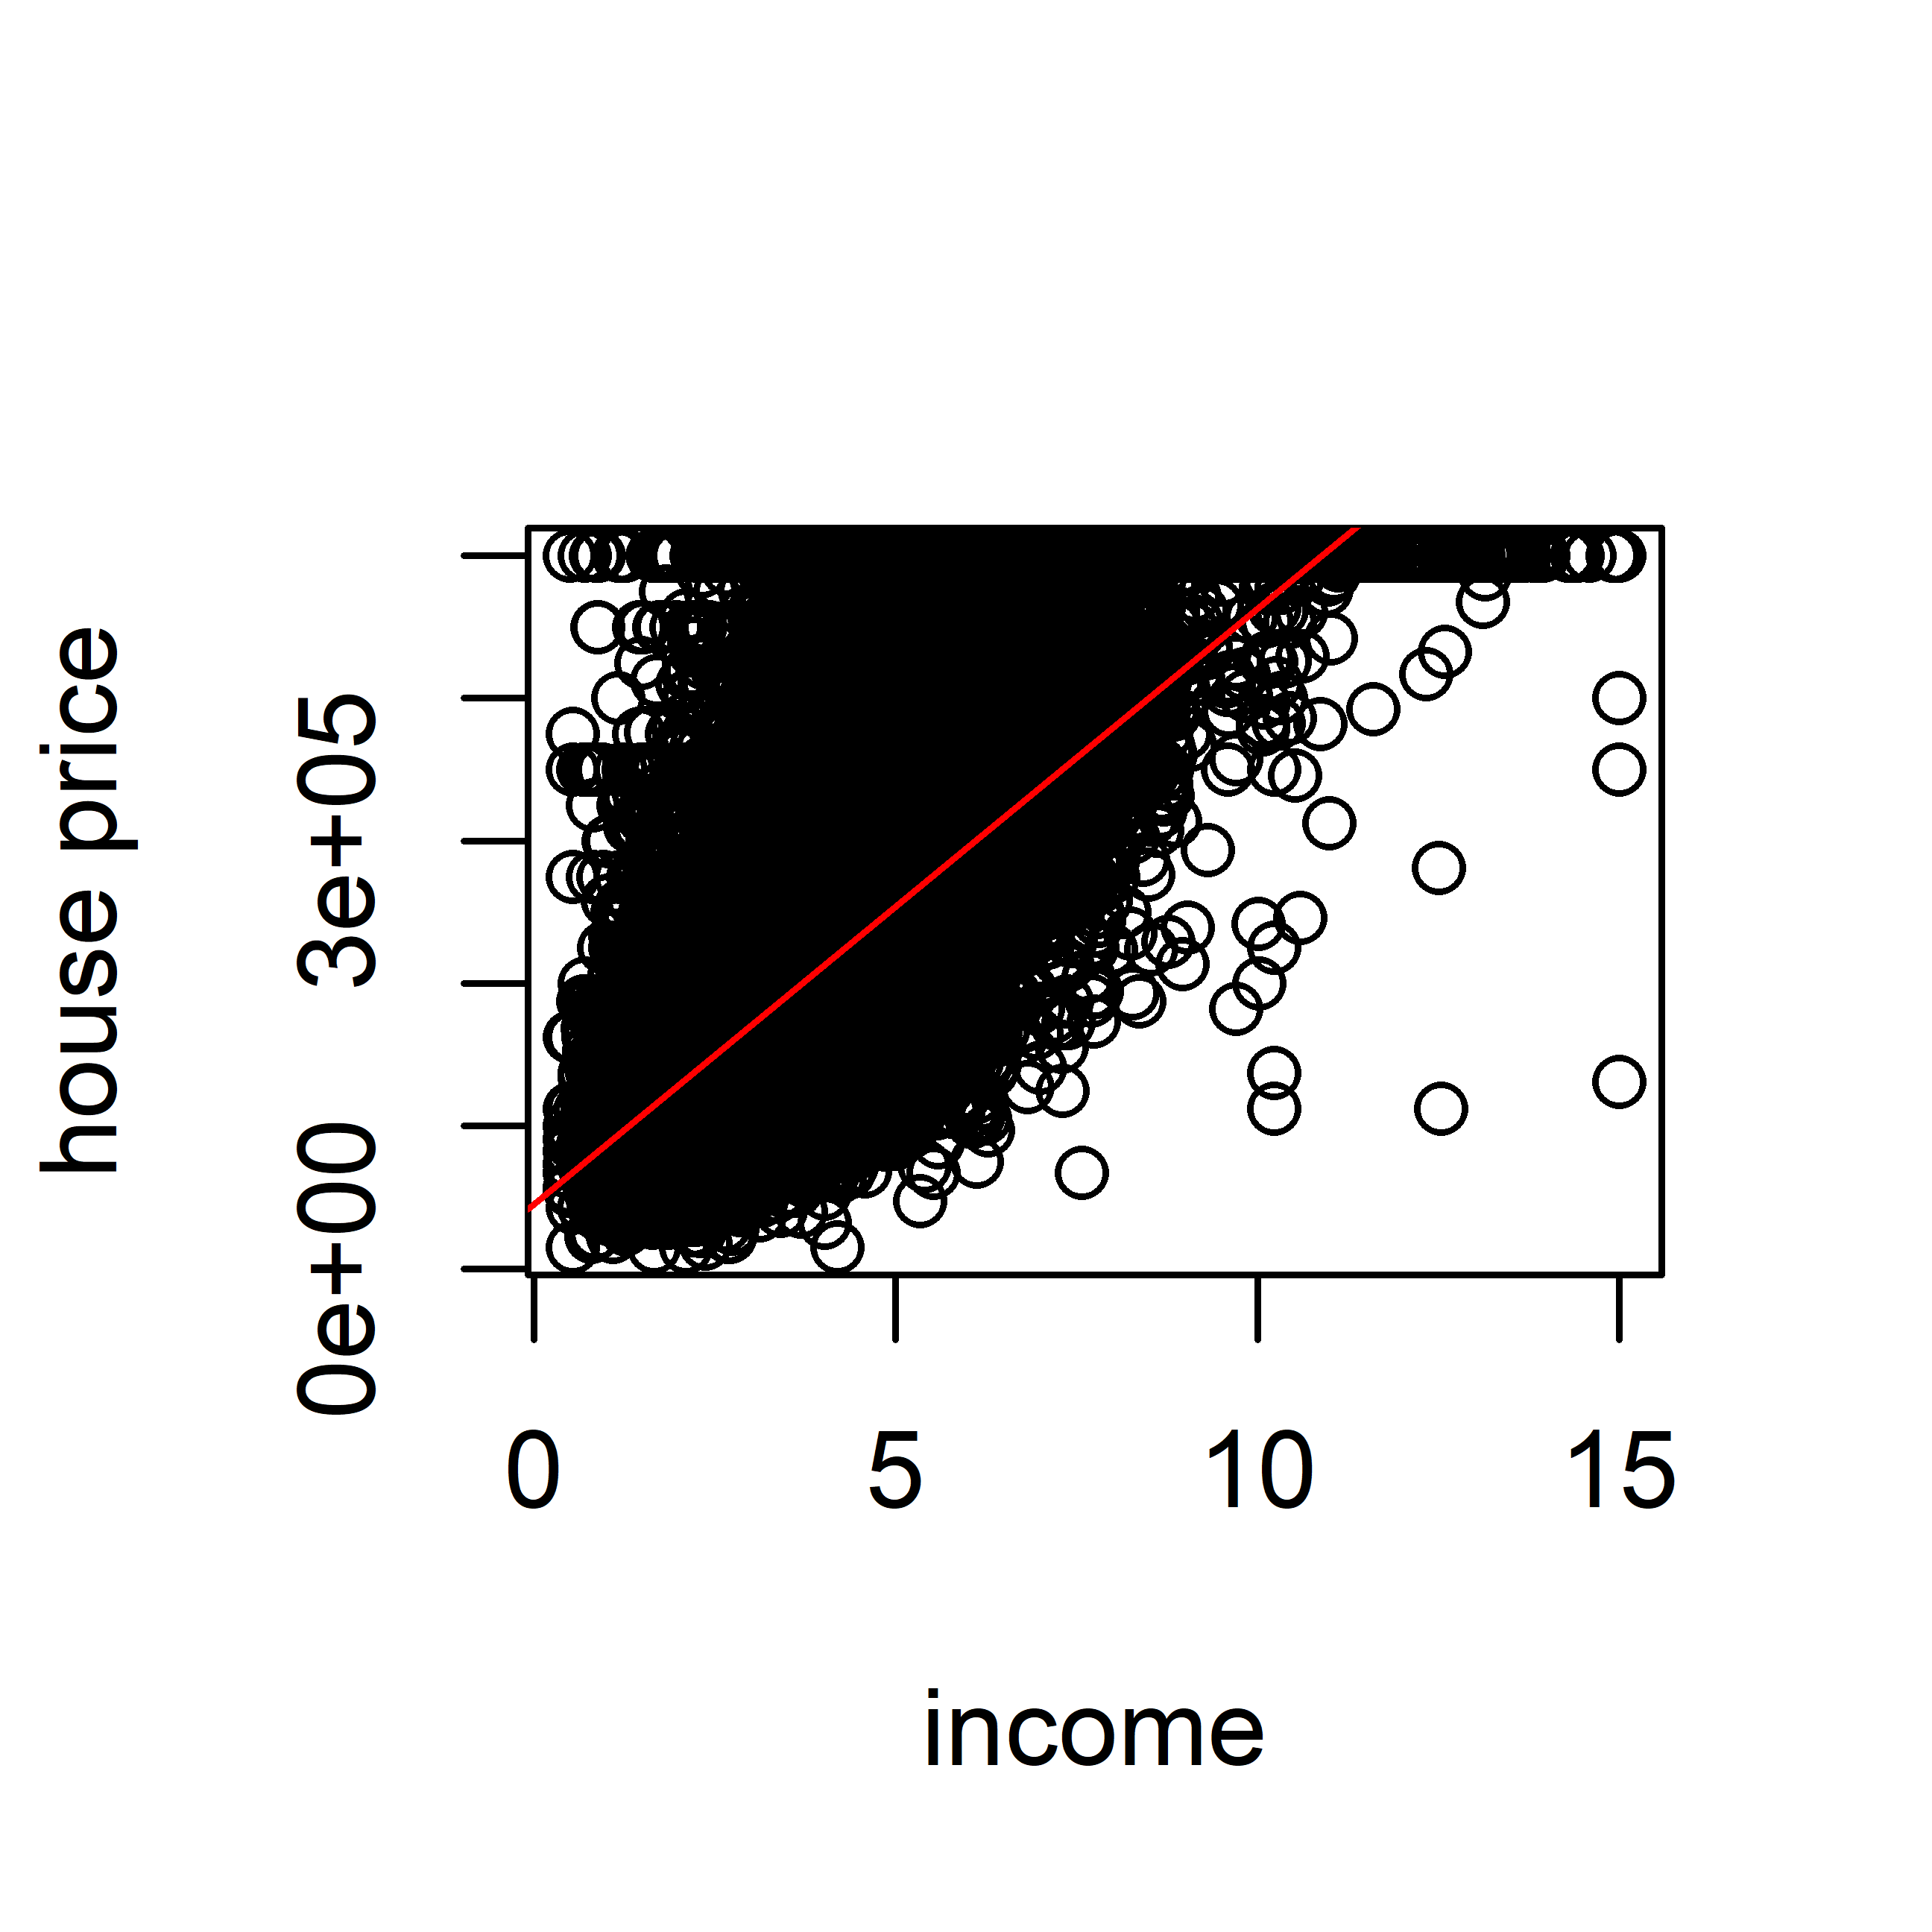
\includegraphics{Bank_files/figure-latex/unnamed-chunk-3-1} \end{center}

\begin{Shaded}
\begin{Highlighting}[]
\CommentTok{\# New grouping variable for duration}
\NormalTok{BankMarketing}\SpecialCharTok{$}\NormalTok{grp.duration }\OtherTok{\textless{}{-}} \FunctionTok{ifelse}\NormalTok{(BankMarketing}\SpecialCharTok{$}\NormalTok{duration }\SpecialCharTok{\textless{}=} \DecValTok{180}\NormalTok{, }\StringTok{\textquotesingle{}0{-}180\textquotesingle{}}\NormalTok{,}
               \FunctionTok{ifelse}\NormalTok{(BankMarketing}\SpecialCharTok{$}\NormalTok{duration }\SpecialCharTok{\textgreater{}=} \DecValTok{320}\NormalTok{, }\StringTok{\textquotesingle{}320+\textquotesingle{}}\NormalTok{, }\StringTok{\textquotesingle{}[181, 319]\textquotesingle{}}\NormalTok{))}
\end{Highlighting}
\end{Shaded}

Now we want to look at some of the categorical and binary features. When
looking at the distribution of contacts performed during the campain, it
is Skewed to the right. This means that groups should be created. For
campaign, the value of 1 contact should be its own group since it has
the highest frequency of observations. Values 2 \& 3 number of contacts
combined have close to the same frequency, so they should be paired
together in their own group. The remaining observations should be
combined into the final group.

When looking at pdays, the value of -1 is an indicator that a client was
not previously contacted before the campaign. Since this makes up most
of the obersvations, it will become its own group. The rest of the
observations were split into groups of 1-200 days and 200 days or more.

The previous variable was also split into 3 groups. The value of 0
contacts is one group since it has the most observations. The values of
1 to 3 contacts is another category since they both make a fair amount
of the observations. Same goes for observations with 4 or more contacts.

All of these bar plots can be seen below.

\begin{Shaded}
\begin{Highlighting}[]
\CommentTok{\# barplot showing the distribution of the campaign variable}
\NormalTok{marketcampaigns }\OtherTok{=} \FunctionTok{table}\NormalTok{(BankMarketing}\SpecialCharTok{$}\NormalTok{campaign)}
\FunctionTok{barplot}\NormalTok{(marketcampaigns, }\AttributeTok{main =} \StringTok{"Distribution of Contacts Performed During Campaign"}\NormalTok{, }\AttributeTok{xlab =} \StringTok{"Number of Contacts"}\NormalTok{)}
\end{Highlighting}
\end{Shaded}

\begin{center}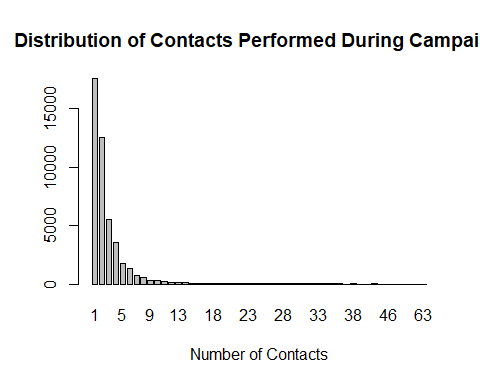
\includegraphics{Bank_files/figure-latex/unnamed-chunk-5-1} \end{center}

\begin{Shaded}
\begin{Highlighting}[]
\CommentTok{\# barplot showing the distribution of the pdays variable}
\NormalTok{dayspassed }\OtherTok{=} \FunctionTok{table}\NormalTok{(BankMarketing}\SpecialCharTok{$}\NormalTok{pdays)}
\FunctionTok{barplot}\NormalTok{(dayspassed, }\AttributeTok{main =} \StringTok{"Distribution of Days Passed After Client Last Contacted (Pdays) "}\NormalTok{, }\AttributeTok{xlab =} \StringTok{"Number of Days"}\NormalTok{)}
\end{Highlighting}
\end{Shaded}

\begin{center}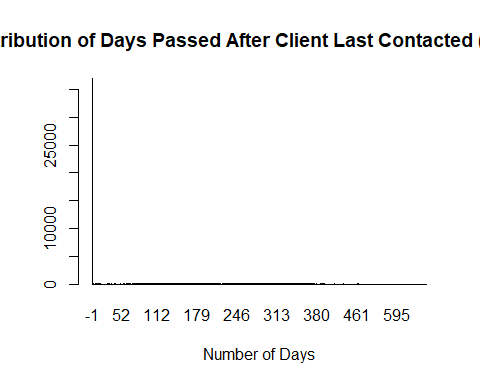
\includegraphics{Bank_files/figure-latex/unnamed-chunk-6-1} \end{center}

\begin{Shaded}
\begin{Highlighting}[]
\CommentTok{\# barplot showing the distribution of the previous variable}
\NormalTok{prev }\OtherTok{=} \FunctionTok{table}\NormalTok{(BankMarketing}\SpecialCharTok{$}\NormalTok{previous)}
\FunctionTok{barplot}\NormalTok{(prev, }\AttributeTok{main =} \StringTok{"Distribution of Previous Contacts"}\NormalTok{, }\AttributeTok{xlab =} \StringTok{"Number of Contacts"}\NormalTok{)}
\end{Highlighting}
\end{Shaded}

\begin{center}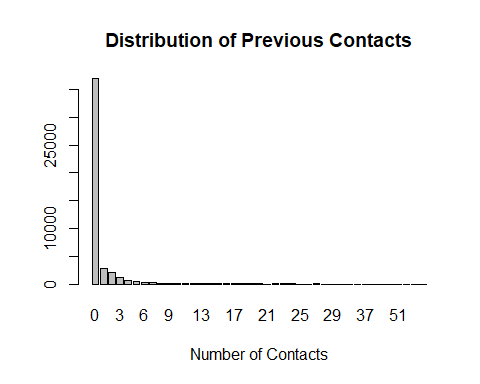
\includegraphics{Bank_files/figure-latex/unnamed-chunk-7-1} \end{center}

These new grouped variables will be used in future model build. The
categories for each variable are as follows:

campaign: 1, 2-3, 4+ pdays: -1, 1-199, 200+ previous: 0, 1-3, 4+

\begin{Shaded}
\begin{Highlighting}[]
\CommentTok{\# New grouping variable for month}
\NormalTok{BankMarketing}\SpecialCharTok{$}\NormalTok{grp.campaign }\OtherTok{\textless{}{-}} \FunctionTok{ifelse}\NormalTok{(BankMarketing}\SpecialCharTok{$}\NormalTok{campaign }\SpecialCharTok{\textless{}=} \DecValTok{1}\NormalTok{, }\StringTok{\textquotesingle{}1\textquotesingle{}}\NormalTok{,}
               \FunctionTok{ifelse}\NormalTok{(BankMarketing}\SpecialCharTok{$}\NormalTok{campaign }\SpecialCharTok{\textgreater{}=} \DecValTok{4}\NormalTok{, }\StringTok{\textquotesingle{}4+\textquotesingle{}}\NormalTok{, }\StringTok{\textquotesingle{}[2, 3]\textquotesingle{}}\NormalTok{))}

\CommentTok{\# New grouping variable for pdays}
\NormalTok{BankMarketing}\SpecialCharTok{$}\NormalTok{grp.pdays }\OtherTok{\textless{}{-}} \FunctionTok{ifelse}\NormalTok{(BankMarketing}\SpecialCharTok{$}\NormalTok{pdays }\SpecialCharTok{\textless{}=} \SpecialCharTok{{-}}\DecValTok{1}\NormalTok{, }\StringTok{\textquotesingle{}Client Not Previously Contacted\textquotesingle{}}\NormalTok{, }\FunctionTok{ifelse}\NormalTok{(BankMarketing}\SpecialCharTok{$}\NormalTok{pdays }\SpecialCharTok{\textgreater{}=} \DecValTok{200}\NormalTok{, }\StringTok{\textquotesingle{}200+\textquotesingle{}}\NormalTok{, }\StringTok{\textquotesingle{}[1, 199]\textquotesingle{}}\NormalTok{))}

\CommentTok{\# New grouping variable for previous}
\NormalTok{BankMarketing}\SpecialCharTok{$}\NormalTok{grp.previous }\OtherTok{\textless{}{-}} \FunctionTok{ifelse}\NormalTok{(BankMarketing}\SpecialCharTok{$}\NormalTok{previous }\SpecialCharTok{\textless{}=} \DecValTok{0}\NormalTok{, }\StringTok{\textquotesingle{}0\textquotesingle{}}\NormalTok{,}
               \FunctionTok{ifelse}\NormalTok{(BankMarketing}\SpecialCharTok{$}\NormalTok{previous }\SpecialCharTok{\textgreater{}} \DecValTok{4}\NormalTok{, }\StringTok{\textquotesingle{}4+\textquotesingle{}}\NormalTok{, }\StringTok{\textquotesingle{}[1,3]\textquotesingle{}}\NormalTok{))}
\end{Highlighting}
\end{Shaded}

Now we move onto categorical varibles.

The categorical variable of month has also been discretized by seasons
since the bar plot below is also skewed for certain months. Also,
handling smaller groups into seasons is easier than hanling 12 months. A
new feature called ``seasons'' was created.

\begin{Shaded}
\begin{Highlighting}[]
\CommentTok{\# barplot showing the distribution of the month variable}
\NormalTok{seasons }\OtherTok{=} \FunctionTok{table}\NormalTok{(BankMarketing}\SpecialCharTok{$}\NormalTok{month)}
\FunctionTok{barplot}\NormalTok{(seasons, }\AttributeTok{main =} \StringTok{"Distribution of Number of Contacts by Month"}\NormalTok{, }\AttributeTok{xlab =} \StringTok{"Number of Contacts"}\NormalTok{)}
\end{Highlighting}
\end{Shaded}

\begin{center}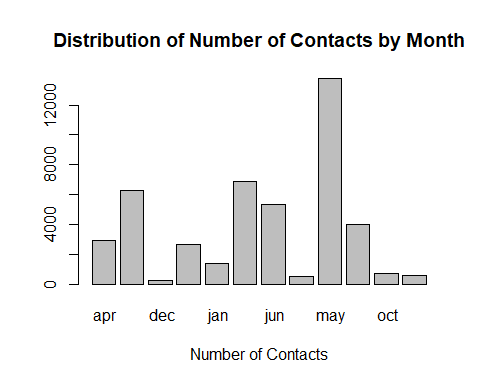
\includegraphics{Bank_files/figure-latex/unnamed-chunk-9-1} \end{center}

\begin{Shaded}
\begin{Highlighting}[]
\CommentTok{\# New grouping variable for month}
\NormalTok{BankMarketing}\SpecialCharTok{$}\NormalTok{grp.month }\OtherTok{\textless{}{-}}  \FunctionTok{ifelse}\NormalTok{((BankMarketing}\SpecialCharTok{$}\NormalTok{month }\SpecialCharTok{==} \StringTok{\textquotesingle{}mar\textquotesingle{}} \SpecialCharTok{|}\NormalTok{ BankMarketing}\SpecialCharTok{$}\NormalTok{month }\SpecialCharTok{==} \StringTok{\textquotesingle{}apr\textquotesingle{}} \SpecialCharTok{|}\NormalTok{ BankMarketing}\SpecialCharTok{$}\NormalTok{month }\SpecialCharTok{==} \StringTok{\textquotesingle{}may\textquotesingle{}}\NormalTok{), }\StringTok{\textquotesingle{}spring\textquotesingle{}}\NormalTok{,}
                            \FunctionTok{ifelse}\NormalTok{((BankMarketing}\SpecialCharTok{$}\NormalTok{month }\SpecialCharTok{==} \StringTok{\textquotesingle{}jun\textquotesingle{}} \SpecialCharTok{|}\NormalTok{ BankMarketing}\SpecialCharTok{$}\NormalTok{month }\SpecialCharTok{==} \StringTok{\textquotesingle{}jul\textquotesingle{}} \SpecialCharTok{|}\NormalTok{ BankMarketing}\SpecialCharTok{$}\NormalTok{month }\SpecialCharTok{==} \StringTok{\textquotesingle{}aug\textquotesingle{}}\NormalTok{), }\StringTok{\textquotesingle{}summer\textquotesingle{}}\NormalTok{, }
                            \FunctionTok{ifelse}\NormalTok{((BankMarketing}\SpecialCharTok{$}\NormalTok{month }\SpecialCharTok{==} \StringTok{\textquotesingle{}sep\textquotesingle{}} \SpecialCharTok{|}\NormalTok{ BankMarketing}\SpecialCharTok{$}\NormalTok{month }\SpecialCharTok{==} \StringTok{\textquotesingle{}oct\textquotesingle{}} \SpecialCharTok{|}\NormalTok{ BankMarketing}\SpecialCharTok{$}\NormalTok{month }\SpecialCharTok{==} \StringTok{\textquotesingle{}nov\textquotesingle{}}\NormalTok{), }\StringTok{\textquotesingle{}fall\textquotesingle{}}\NormalTok{, }\StringTok{\textquotesingle{}winter\textquotesingle{}}\NormalTok{)))}
\end{Highlighting}
\end{Shaded}

\begin{Shaded}
\begin{Highlighting}[]
\CommentTok{\# barplot showing the distribution of the job variable}
\NormalTok{jobcategory }\OtherTok{=} \FunctionTok{table}\NormalTok{(BankMarketing}\SpecialCharTok{$}\NormalTok{job)}
\FunctionTok{barplot}\NormalTok{(jobcategory, }\AttributeTok{main =} \StringTok{"Distribution of Job Type"}\NormalTok{, }\AttributeTok{xlab =} \StringTok{"Number of Clients in Each Job"}\NormalTok{)}
\end{Highlighting}
\end{Shaded}

\begin{center}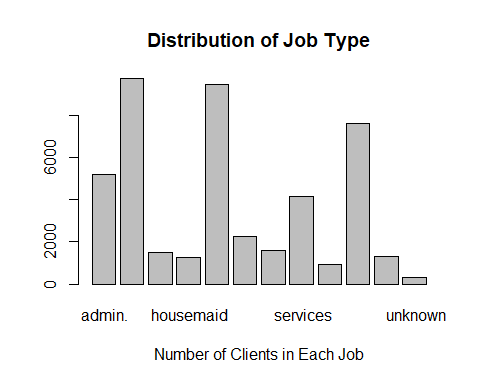
\includegraphics{Bank_files/figure-latex/unnamed-chunk-11-1} \end{center}

\begin{Shaded}
\begin{Highlighting}[]
\CommentTok{\# New grouping variable for job}
\NormalTok{BankMarketing}\SpecialCharTok{$}\NormalTok{grp.job }\OtherTok{=} \FunctionTok{ifelse}\NormalTok{(BankMarketing}\SpecialCharTok{$}\NormalTok{job }\SpecialCharTok{==} \StringTok{" unknown"}\NormalTok{, }\StringTok{"not working"}\NormalTok{, }\FunctionTok{ifelse}\NormalTok{(BankMarketing}\SpecialCharTok{$}\NormalTok{job }\SpecialCharTok{==} \StringTok{" unemployed"}\NormalTok{, }\StringTok{"not working"}\NormalTok{, }\FunctionTok{ifelse}\NormalTok{(BankMarketing}\SpecialCharTok{$}\NormalTok{job }\SpecialCharTok{==} \StringTok{" retired"}\NormalTok{, }\StringTok{"not working"}\NormalTok{, }\FunctionTok{ifelse}\NormalTok{(BankMarketing}\SpecialCharTok{$}\NormalTok{job }\SpecialCharTok{==} \StringTok{" blue{-}collar"}\NormalTok{, }\StringTok{"workers"}\NormalTok{, }\FunctionTok{ifelse}\NormalTok{(BankMarketing}\SpecialCharTok{$}\NormalTok{job }\SpecialCharTok{==} \StringTok{" entrepreneur"}\NormalTok{, }\StringTok{"bosses"}\NormalTok{, }\FunctionTok{ifelse}\NormalTok{(BankMarketing}\SpecialCharTok{$}\NormalTok{job }\SpecialCharTok{==} \StringTok{" housemaid"}\NormalTok{, }\StringTok{"workers"}\NormalTok{, }\FunctionTok{ifelse}\NormalTok{(BankMarketing}\SpecialCharTok{$}\NormalTok{job }\SpecialCharTok{==} \StringTok{" management"}\NormalTok{, }\StringTok{"bosses"}\NormalTok{, }\FunctionTok{ifelse}\NormalTok{(BankMarketing}\SpecialCharTok{$}\NormalTok{job }\SpecialCharTok{==} \StringTok{" self{-}employed"}\NormalTok{, }\StringTok{"bosses"}\NormalTok{, }\FunctionTok{ifelse}\NormalTok{(BankMarketing}\SpecialCharTok{$}\NormalTok{job }\SpecialCharTok{==} \StringTok{" services"}\NormalTok{, }\StringTok{"white{-}collar"}\NormalTok{, }\FunctionTok{ifelse}\NormalTok{(BankMarketing}\SpecialCharTok{$}\NormalTok{job }\SpecialCharTok{==} \StringTok{" technician"}\NormalTok{, }\StringTok{"white{-}collar"}\NormalTok{, }\FunctionTok{ifelse}\NormalTok{(BankMarketing}\SpecialCharTok{$}\NormalTok{job }\SpecialCharTok{==} \StringTok{" student"}\NormalTok{, }\StringTok{"not working"}\NormalTok{, }\StringTok{"white{-}collar"}\NormalTok{)))))))))))}
\end{Highlighting}
\end{Shaded}

Now that we have Now that the variables have been discretized, and
created new variables, the dataset now must be cleaned to reflect those
changes.

\begin{Shaded}
\begin{Highlighting}[]
\CommentTok{\# Assembling the discretized variables and other variables to make the modeling data set}
\NormalTok{var.names }\OtherTok{=} \FunctionTok{c}\NormalTok{(}\StringTok{"age"}\NormalTok{, }\StringTok{"balance"}\NormalTok{, }\StringTok{"day"}\NormalTok{, }\StringTok{"grp.job"}\NormalTok{, }\StringTok{"marital"}\NormalTok{, }\StringTok{"education"}\NormalTok{, }\StringTok{"default"}\NormalTok{, }\StringTok{"housing"}\NormalTok{, }\StringTok{"loan"}\NormalTok{, }\StringTok{"contact"}\NormalTok{, }\StringTok{"grp.month"}\NormalTok{, }\StringTok{"grp.duration"}\NormalTok{, }\StringTok{"grp.campaign"}\NormalTok{, }\StringTok{"grp.pdays"}\NormalTok{, }\StringTok{"grp.previous"}\NormalTok{, }\StringTok{"poutcome"}\NormalTok{, }\StringTok{"y"}\NormalTok{) }

\NormalTok{BankMarketingCampaign }\OtherTok{\textless{}{-}}\NormalTok{ BankMarketing[, var.names]}
\CommentTok{\#BankMarketingCampaign = BankMarketing[,var.names]}
\end{Highlighting}
\end{Shaded}

\subsection{Assessing Pairwised
Relationship}\label{assessing-pairwised-relationship}

We want to see if there is any linear association between the numeric
variables. A Pairwise scatter plot like below, is a good visual. This
scatterplot blow looks at the data.

\begin{Shaded}
\begin{Highlighting}[]
\CommentTok{\# Pair{-}wise scatter plot for numeric variables}
\FunctionTok{ggpairs}\NormalTok{(BankMarketingCampaign,  }\CommentTok{\# Data frame}
        \AttributeTok{columns =} \DecValTok{1}\SpecialCharTok{:}\DecValTok{3}\NormalTok{,  }\CommentTok{\# Columns}
        \FunctionTok{aes}\NormalTok{(}\AttributeTok{color =}\NormalTok{ y,  }\CommentTok{\# Color by group (cat. variable)}
            \AttributeTok{alpha =} \FloatTok{0.5}\NormalTok{))}
\end{Highlighting}
\end{Shaded}

\begin{center}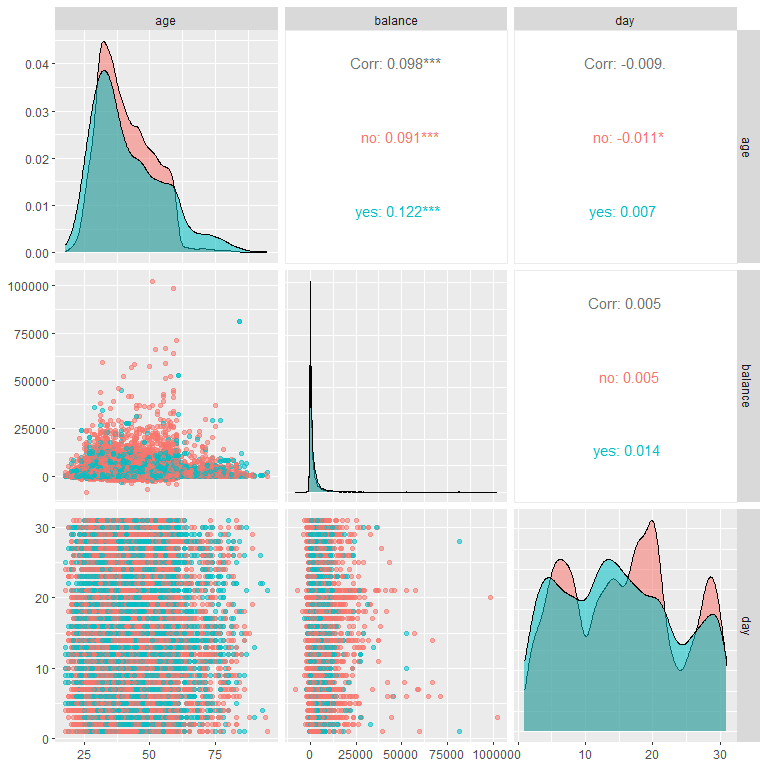
\includegraphics{Bank_files/figure-latex/unnamed-chunk-13-1} \end{center}

We see that none of the numeric variables appear to be significantly
correlated when looking at the numbers. But, the stacked density cures
and no completely overlapping, indicating a week correlation between the
numeric variables and our response `y'. The strongest but 'weak
correlation we can see through the plots is age and balance.

Now that we looked at the numeric variables, we can turn the attention
to categorical variables and dependency. In order to see dependency,
mosaic plots will be shown below.

\begin{Shaded}
\begin{Highlighting}[]
\CommentTok{\# Mosaic plots to show categorical variable dependency to the response.}
\FunctionTok{par}\NormalTok{(}\AttributeTok{mfrow =} \FunctionTok{c}\NormalTok{(}\DecValTok{2}\NormalTok{,}\DecValTok{2}\NormalTok{))}
\FunctionTok{mosaicplot}\NormalTok{(grp.job }\SpecialCharTok{\textasciitilde{}}\NormalTok{ y, }\AttributeTok{data=}\NormalTok{BankMarketingCampaign,}\AttributeTok{col=}\FunctionTok{c}\NormalTok{(}\StringTok{"Blue"}\NormalTok{,}\StringTok{"Red"}\NormalTok{), }\AttributeTok{main=}\StringTok{"job vs term deposit "}\NormalTok{)}
\FunctionTok{mosaicplot}\NormalTok{(marital }\SpecialCharTok{\textasciitilde{}}\NormalTok{ y, }\AttributeTok{data=}\NormalTok{BankMarketingCampaign,}\AttributeTok{col=}\FunctionTok{c}\NormalTok{(}\StringTok{"Blue"}\NormalTok{,}\StringTok{"Red"}\NormalTok{), }\AttributeTok{main=}\StringTok{"marital vs term deposit "}\NormalTok{)}
\FunctionTok{mosaicplot}\NormalTok{(education }\SpecialCharTok{\textasciitilde{}}\NormalTok{ y, }\AttributeTok{data=}\NormalTok{BankMarketingCampaign,}\AttributeTok{col=}\FunctionTok{c}\NormalTok{(}\StringTok{"Blue"}\NormalTok{,}\StringTok{"Red"}\NormalTok{), }\AttributeTok{main=}\StringTok{"education vs term deposit "}\NormalTok{)}
\FunctionTok{mosaicplot}\NormalTok{(default }\SpecialCharTok{\textasciitilde{}}\NormalTok{ y, }\AttributeTok{data=}\NormalTok{BankMarketingCampaign,}\AttributeTok{col=}\FunctionTok{c}\NormalTok{(}\StringTok{"Blue"}\NormalTok{,}\StringTok{"Red"}\NormalTok{), }\AttributeTok{main=}\StringTok{"default vs term deposit "}\NormalTok{)}
\end{Highlighting}
\end{Shaded}

\begin{center}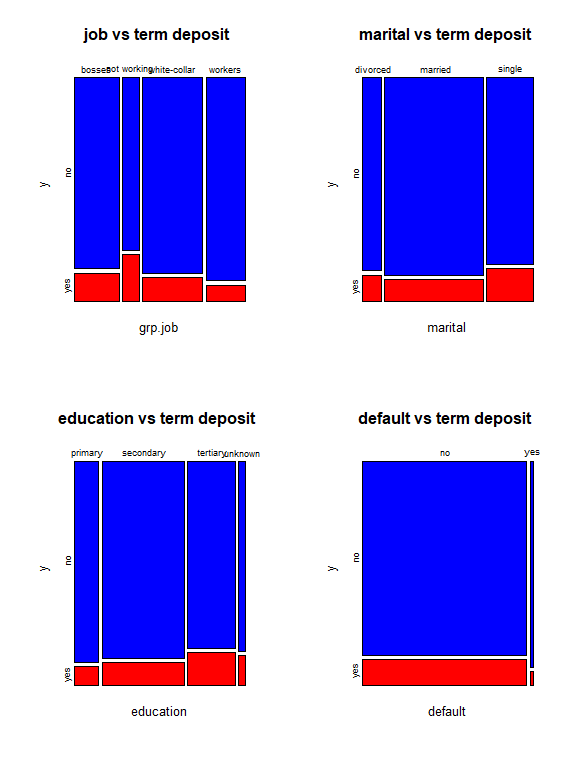
\includegraphics{Bank_files/figure-latex/unnamed-chunk-14-1} \end{center}

\begin{Shaded}
\begin{Highlighting}[]
\CommentTok{\# Mosaic plots to show categorical variable dependency to the response.}
\FunctionTok{par}\NormalTok{(}\AttributeTok{mfrow =} \FunctionTok{c}\NormalTok{(}\DecValTok{2}\NormalTok{,}\DecValTok{2}\NormalTok{))}
\FunctionTok{mosaicplot}\NormalTok{(housing }\SpecialCharTok{\textasciitilde{}}\NormalTok{ y, }\AttributeTok{data=}\NormalTok{BankMarketingCampaign,}\AttributeTok{col=}\FunctionTok{c}\NormalTok{(}\StringTok{"Blue"}\NormalTok{,}\StringTok{"Red"}\NormalTok{), }\AttributeTok{main=}\StringTok{"housing vs term deposit "}\NormalTok{)}
\FunctionTok{mosaicplot}\NormalTok{(loan }\SpecialCharTok{\textasciitilde{}}\NormalTok{ y, }\AttributeTok{data=}\NormalTok{BankMarketingCampaign,}\AttributeTok{col=}\FunctionTok{c}\NormalTok{(}\StringTok{"Blue"}\NormalTok{,}\StringTok{"Red"}\NormalTok{), }\AttributeTok{main=}\StringTok{"loan vs term deposit "}\NormalTok{)}
\FunctionTok{mosaicplot}\NormalTok{(contact }\SpecialCharTok{\textasciitilde{}}\NormalTok{ y, }\AttributeTok{data=}\NormalTok{BankMarketingCampaign,}\AttributeTok{col=}\FunctionTok{c}\NormalTok{(}\StringTok{"Blue"}\NormalTok{,}\StringTok{"Red"}\NormalTok{), }\AttributeTok{main=}\StringTok{"contact vs term deposit "}\NormalTok{)}
\FunctionTok{mosaicplot}\NormalTok{(grp.month }\SpecialCharTok{\textasciitilde{}}\NormalTok{ y, }\AttributeTok{data=}\NormalTok{BankMarketingCampaign,}\AttributeTok{col=}\FunctionTok{c}\NormalTok{(}\StringTok{"Blue"}\NormalTok{,}\StringTok{"Red"}\NormalTok{), }\AttributeTok{main=}\StringTok{"month vs term deposit "}\NormalTok{)}
\end{Highlighting}
\end{Shaded}

\begin{center}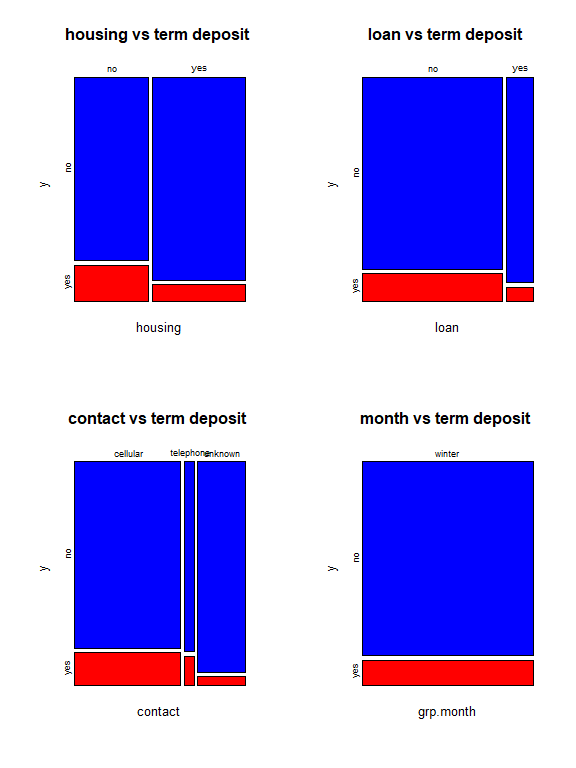
\includegraphics{Bank_files/figure-latex/unnamed-chunk-15-1} \end{center}

\begin{Shaded}
\begin{Highlighting}[]
\CommentTok{\# Mosaic plots to show categorical variable dependency to the response.}
\FunctionTok{par}\NormalTok{(}\AttributeTok{mfrow =} \FunctionTok{c}\NormalTok{(}\DecValTok{3}\NormalTok{,}\DecValTok{2}\NormalTok{))}
\FunctionTok{mosaicplot}\NormalTok{(grp.duration }\SpecialCharTok{\textasciitilde{}}\NormalTok{ y, }\AttributeTok{data=}\NormalTok{BankMarketingCampaign,}\AttributeTok{col=}\FunctionTok{c}\NormalTok{(}\StringTok{"Blue"}\NormalTok{,}\StringTok{"Red"}\NormalTok{), }\AttributeTok{main=}\StringTok{"duration vs term deposit "}\NormalTok{)}
\FunctionTok{mosaicplot}\NormalTok{(grp.campaign }\SpecialCharTok{\textasciitilde{}}\NormalTok{ y, }\AttributeTok{data=}\NormalTok{BankMarketingCampaign,}\AttributeTok{col=}\FunctionTok{c}\NormalTok{(}\StringTok{"Blue"}\NormalTok{,}\StringTok{"Red"}\NormalTok{), }\AttributeTok{main=}\StringTok{"campaign vs term deposit "}\NormalTok{)}
\FunctionTok{mosaicplot}\NormalTok{(grp.pdays }\SpecialCharTok{\textasciitilde{}}\NormalTok{ y, }\AttributeTok{data=}\NormalTok{BankMarketingCampaign,}\AttributeTok{col=}\FunctionTok{c}\NormalTok{(}\StringTok{"Blue"}\NormalTok{,}\StringTok{"Red"}\NormalTok{), }\AttributeTok{main=}\StringTok{"pdays vs term deposit "}\NormalTok{)}
\FunctionTok{mosaicplot}\NormalTok{(grp.previous }\SpecialCharTok{\textasciitilde{}}\NormalTok{ y, }\AttributeTok{data=}\NormalTok{BankMarketingCampaign,}\AttributeTok{col=}\FunctionTok{c}\NormalTok{(}\StringTok{"Blue"}\NormalTok{,}\StringTok{"Red"}\NormalTok{), }\AttributeTok{main=}\StringTok{"previous vs term deposit "}\NormalTok{)}
\FunctionTok{mosaicplot}\NormalTok{(poutcome }\SpecialCharTok{\textasciitilde{}}\NormalTok{ y, }\AttributeTok{data=}\NormalTok{BankMarketingCampaign,}\AttributeTok{col=}\FunctionTok{c}\NormalTok{(}\StringTok{"Blue"}\NormalTok{,}\StringTok{"Red"}\NormalTok{), }\AttributeTok{main=}\StringTok{"poutcome vs term deposit "}\NormalTok{)}
\end{Highlighting}
\end{Shaded}

\begin{center}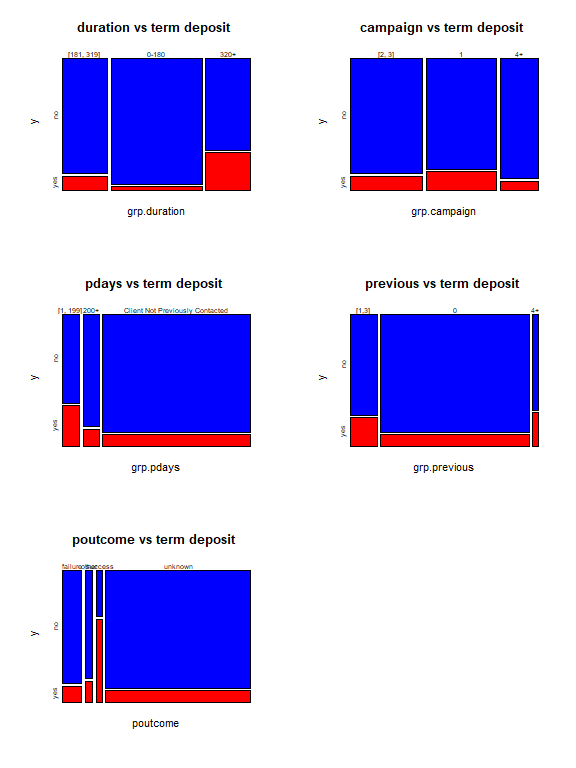
\includegraphics{Bank_files/figure-latex/unnamed-chunk-16-1} \end{center}

\section{Linear Regression Modeling}\label{linear-regression-modeling}

We can use a linear model for finding association variables and the
duration of the phone calls in seconds.The variable, duration, which
tells tells how long the phone call last is the reponse response
variable.

Before we can model, all binary and categorical variables must be
changes to numerical dummy variables. This is done below.

\begin{Shaded}
\begin{Highlighting}[]
\CommentTok{\# Create numerical value labels for categorical variables}
\NormalTok{BankMarketingCampaign}\SpecialCharTok{$}\NormalTok{y }\OtherTok{\textless{}{-}} \FunctionTok{factor}\NormalTok{(BankMarketingCampaign}\SpecialCharTok{$}\NormalTok{y, }\AttributeTok{levels =} \FunctionTok{c}\NormalTok{(}\StringTok{" no"}\NormalTok{, }\StringTok{" yes"}\NormalTok{), }\AttributeTok{labels =} \FunctionTok{c}\NormalTok{(}\StringTok{"0"}\NormalTok{, }\StringTok{"1"}\NormalTok{))}

\NormalTok{BankMarketingCampaign}\SpecialCharTok{$}\NormalTok{grp.job }\OtherTok{\textless{}{-}} \FunctionTok{factor}\NormalTok{(BankMarketingCampaign}\SpecialCharTok{$}\NormalTok{grp.job, }\AttributeTok{levels =} \FunctionTok{c}\NormalTok{(}\StringTok{"not working"}\NormalTok{, }\StringTok{"workers"}\NormalTok{, }\StringTok{"bosses"}\NormalTok{, }\StringTok{"white{-}collar"}\NormalTok{), }\AttributeTok{labels =} \FunctionTok{c}\NormalTok{(}\StringTok{"0"}\NormalTok{, }\StringTok{"1"}\NormalTok{, }\StringTok{"2"}\NormalTok{, }\StringTok{"3"}\NormalTok{))}

\NormalTok{BankMarketingCampaign}\SpecialCharTok{$}\NormalTok{marital }\OtherTok{\textless{}{-}} \FunctionTok{factor}\NormalTok{(BankMarketingCampaign}\SpecialCharTok{$}\NormalTok{marital, }\AttributeTok{levels =} \FunctionTok{c}\NormalTok{(}\StringTok{" divorced"}\NormalTok{, }\StringTok{" single"}\NormalTok{, }\StringTok{" married"}\NormalTok{), }\AttributeTok{labels =} \FunctionTok{c}\NormalTok{(}\StringTok{"0"}\NormalTok{, }\StringTok{"1"}\NormalTok{, }\StringTok{"2"}\NormalTok{))}

\NormalTok{BankMarketingCampaign}\SpecialCharTok{$}\NormalTok{education }\OtherTok{\textless{}{-}} \FunctionTok{factor}\NormalTok{(BankMarketingCampaign}\SpecialCharTok{$}\NormalTok{education, }\AttributeTok{levels =} \FunctionTok{c}\NormalTok{(}\StringTok{" unknown"}\NormalTok{, }\StringTok{" primary"}\NormalTok{, }\StringTok{" secondary"}\NormalTok{, }\StringTok{" tertiary"}\NormalTok{), }\AttributeTok{labels =} \FunctionTok{c}\NormalTok{(}\StringTok{"0"}\NormalTok{, }\StringTok{"1"}\NormalTok{, }\StringTok{"2"}\NormalTok{, }\StringTok{"3"}\NormalTok{))}
  
\NormalTok{BankMarketingCampaign}\SpecialCharTok{$}\NormalTok{housing }\OtherTok{\textless{}{-}} \FunctionTok{factor}\NormalTok{(BankMarketingCampaign}\SpecialCharTok{$}\NormalTok{housing, }\AttributeTok{levels =} \FunctionTok{c}\NormalTok{(}\StringTok{" no"}\NormalTok{, }\StringTok{" yes"}\NormalTok{), }\AttributeTok{labels =} \FunctionTok{c}\NormalTok{(}\StringTok{"0"}\NormalTok{, }\StringTok{"1"}\NormalTok{))}
  
\NormalTok{BankMarketingCampaign}\SpecialCharTok{$}\NormalTok{loan }\OtherTok{\textless{}{-}} \FunctionTok{factor}\NormalTok{(BankMarketingCampaign}\SpecialCharTok{$}\NormalTok{loan, }\AttributeTok{levels =} \FunctionTok{c}\NormalTok{(}\StringTok{" no"}\NormalTok{, }\StringTok{" yes"}\NormalTok{), }\AttributeTok{labels =} \FunctionTok{c}\NormalTok{(}\StringTok{"0"}\NormalTok{, }\StringTok{"1"}\NormalTok{))}
\NormalTok{BankMarketingCampaign}\SpecialCharTok{$}\NormalTok{default }\OtherTok{\textless{}{-}} \FunctionTok{factor}\NormalTok{(BankMarketingCampaign}\SpecialCharTok{$}\NormalTok{default, }\AttributeTok{levels =} \FunctionTok{c}\NormalTok{(}\StringTok{" no"}\NormalTok{, }\StringTok{" yes"}\NormalTok{), }\AttributeTok{labels =} \FunctionTok{c}\NormalTok{(}\StringTok{"0"}\NormalTok{, }\StringTok{"1"}\NormalTok{))}
\NormalTok{BankMarketingCampaign}\SpecialCharTok{$}\NormalTok{contact }\OtherTok{\textless{}{-}} \FunctionTok{factor}\NormalTok{(BankMarketingCampaign}\SpecialCharTok{$}\NormalTok{contact, }\AttributeTok{levels =} \FunctionTok{c}\NormalTok{(}\StringTok{" unknown"}\NormalTok{, }\StringTok{" telephone"}\NormalTok{, }\StringTok{" cellular"}\NormalTok{), }\AttributeTok{labels =} \FunctionTok{c}\NormalTok{(}\StringTok{"0"}\NormalTok{, }\StringTok{"1"}\NormalTok{, }\StringTok{"2"}\NormalTok{))}

\NormalTok{BankMarketingCampaign}\SpecialCharTok{$}\NormalTok{grp.month }\OtherTok{\textless{}{-}} \FunctionTok{factor}\NormalTok{(BankMarketingCampaign}\SpecialCharTok{$}\NormalTok{grp.month, }\AttributeTok{levels =} \FunctionTok{c}\NormalTok{(}\StringTok{"winter"}\NormalTok{, }\StringTok{"spring"}\NormalTok{, }\StringTok{"summer"}\NormalTok{, }\StringTok{"fall"}\NormalTok{), }\AttributeTok{labels =} \FunctionTok{c}\NormalTok{(}\StringTok{"0"}\NormalTok{, }\StringTok{"1"}\NormalTok{, }\StringTok{"2"}\NormalTok{, }\StringTok{"3"}\NormalTok{))}

\NormalTok{BankMarketingCampaign}\SpecialCharTok{$}\NormalTok{grp.duration }\OtherTok{\textless{}{-}} \FunctionTok{factor}\NormalTok{(BankMarketingCampaign}\SpecialCharTok{$}\NormalTok{grp.duration, }\AttributeTok{levels =} \FunctionTok{c}\NormalTok{(}\StringTok{"0{-}180"}\NormalTok{, }\StringTok{"[181, 319]"}\NormalTok{, }\StringTok{"320+"}\NormalTok{), }\AttributeTok{labels =} \FunctionTok{c}\NormalTok{(}\StringTok{"0"}\NormalTok{, }\StringTok{"1"}\NormalTok{, }\StringTok{"2"}\NormalTok{))}
  
\NormalTok{BankMarketingCampaign}\SpecialCharTok{$}\NormalTok{grp.campaign }\OtherTok{\textless{}{-}} \FunctionTok{factor}\NormalTok{(BankMarketingCampaign}\SpecialCharTok{$}\NormalTok{grp.campaign, }\AttributeTok{levels =} \FunctionTok{c}\NormalTok{(}\StringTok{"1"}\NormalTok{, }\StringTok{"[2, 3]"}\NormalTok{, }\StringTok{"4+"}\NormalTok{), }\AttributeTok{labels =} \FunctionTok{c}\NormalTok{(}\StringTok{"0"}\NormalTok{, }\StringTok{"1"}\NormalTok{, }\StringTok{"2"}\NormalTok{))}
  
\NormalTok{BankMarketingCampaign}\SpecialCharTok{$}\NormalTok{grp.pdays }\OtherTok{\textless{}{-}} \FunctionTok{factor}\NormalTok{(BankMarketingCampaign}\SpecialCharTok{$}\NormalTok{grp.pdays, }\AttributeTok{levels =} \FunctionTok{c}\NormalTok{(}\StringTok{"Client Not Previously Contacted"}\NormalTok{, }\StringTok{"[1, 199]"}\NormalTok{, }\StringTok{"200+"}\NormalTok{), }\AttributeTok{labels =} \FunctionTok{c}\NormalTok{(}\StringTok{"0"}\NormalTok{, }\StringTok{"1"}\NormalTok{, }\StringTok{"2"}\NormalTok{))}
  
\NormalTok{BankMarketingCampaign}\SpecialCharTok{$}\NormalTok{grp.previous }\OtherTok{\textless{}{-}} \FunctionTok{factor}\NormalTok{(BankMarketingCampaign}\SpecialCharTok{$}\NormalTok{grp.previous, }\AttributeTok{levels =} \FunctionTok{c}\NormalTok{(}\StringTok{"0"}\NormalTok{, }\StringTok{"[1,3]"}\NormalTok{, }\StringTok{"4+"}\NormalTok{), }\AttributeTok{labels =} \FunctionTok{c}\NormalTok{(}\StringTok{"0"}\NormalTok{, }\StringTok{"1"}\NormalTok{, }\StringTok{"2"}\NormalTok{))}
  
\NormalTok{BankMarketingCampaign}\SpecialCharTok{$}\NormalTok{poutcome }\OtherTok{\textless{}{-}} \FunctionTok{factor}\NormalTok{(BankMarketingCampaign}\SpecialCharTok{$}\NormalTok{poutcome, }\AttributeTok{levels =} \FunctionTok{c}\NormalTok{(}\StringTok{" unknown"}\NormalTok{, }\StringTok{" success"}\NormalTok{, }\StringTok{" failure"}\NormalTok{, }\StringTok{"  other"}\NormalTok{), }\AttributeTok{labels =} \FunctionTok{c}\NormalTok{(}\StringTok{"0"}\NormalTok{, }\StringTok{"1"}\NormalTok{, }\StringTok{"2"}\NormalTok{, }\StringTok{"3"}\NormalTok{))}
\end{Highlighting}
\end{Shaded}

\begin{Shaded}
\begin{Highlighting}[]
\CommentTok{\#Linear Dataset}
\NormalTok{BankMarketingL }\OtherTok{\textless{}{-}}\NormalTok{ BankMarketingCampaign }\SpecialCharTok{\%\textgreater{}\%}
   \FunctionTok{mutate}\NormalTok{(}\AttributeTok{y =}\NormalTok{ BankMarketingCampaign}\SpecialCharTok{$}\NormalTok{y, }
          \AttributeTok{age=}\NormalTok{BankMarketingCampaign}\SpecialCharTok{$}\NormalTok{age,}
          \AttributeTok{balance=}\NormalTok{BankMarketingCampaign}\SpecialCharTok{$}\NormalTok{balance,}
          \AttributeTok{day =}\NormalTok{ BankMarketingCampaign}\SpecialCharTok{$}\NormalTok{day,}
         \AttributeTok{grp.job =}\NormalTok{ BankMarketingCampaign}\SpecialCharTok{$}\NormalTok{grp.job,}
         \AttributeTok{marital =}\NormalTok{ BankMarketingCampaign}\SpecialCharTok{$}\NormalTok{marital,}
         \AttributeTok{education =}\NormalTok{ BankMarketingCampaign}\SpecialCharTok{$}\NormalTok{education,}
         \AttributeTok{housing =}\NormalTok{ BankMarketingCampaign}\SpecialCharTok{$}\NormalTok{housing,}
         \AttributeTok{loan =}\NormalTok{ BankMarketingCampaign}\SpecialCharTok{$}\NormalTok{loan,}
         \AttributeTok{default =}\NormalTok{ BankMarketingCampaign}\SpecialCharTok{$}\NormalTok{default,}
         \AttributeTok{contact=}\NormalTok{BankMarketingCampaign}\SpecialCharTok{$}\NormalTok{contact,}
         \AttributeTok{grp.campaign =}\NormalTok{ BankMarketingCampaign}\SpecialCharTok{$}\NormalTok{grp.campaign,}
         \AttributeTok{grp.pdays =}\NormalTok{BankMarketingCampaign}\SpecialCharTok{$}\NormalTok{grp.pdays,}
         \AttributeTok{grp.previous =}\NormalTok{ BankMarketingCampaign}\SpecialCharTok{$}\NormalTok{grp.previous,}
         \AttributeTok{poutcome =}\NormalTok{ BankMarketingCampaign}\SpecialCharTok{$}\NormalTok{poutcome, }
         \AttributeTok{duration =}\NormalTok{ BankMarketing}\SpecialCharTok{$}\NormalTok{duration)}

\NormalTok{BankMarketingL }\OtherTok{\textless{}{-}}\NormalTok{ BankMarketingL[BankMarketingL}\SpecialCharTok{$}\NormalTok{duration }\SpecialCharTok{\textgreater{}} \DecValTok{0}\NormalTok{, ]}
\end{Highlighting}
\end{Shaded}

\subsection{Create Candidate Models}\label{create-candidate-models}

The full/initial model containing all of the predictor variables will be
made first, with `duration' (length of call in seconds) as the response.
The variables balance and default are not included since our EDA showed
that removing them from the model might help the results.

\begin{Shaded}
\begin{Highlighting}[]
\CommentTok{\# Create the initial full model}
\NormalTok{initial.model }\OtherTok{=}\FunctionTok{lm}\NormalTok{(duration }\SpecialCharTok{\textasciitilde{}}\NormalTok{ age }\SpecialCharTok{+}\NormalTok{ balance }\SpecialCharTok{+}\NormalTok{ day }\SpecialCharTok{+}\NormalTok{ grp.job }\SpecialCharTok{+}\NormalTok{ marital }\SpecialCharTok{+}\NormalTok{ education }\SpecialCharTok{+}\NormalTok{ default }\SpecialCharTok{+}\NormalTok{ housing }\SpecialCharTok{+}\NormalTok{ loan }\SpecialCharTok{+}\NormalTok{ contact }\SpecialCharTok{+}\NormalTok{ grp.campaign}\SpecialCharTok{+}\NormalTok{grp.pdays}\SpecialCharTok{+}\NormalTok{grp.previous}\SpecialCharTok{+}\NormalTok{poutcome, }\AttributeTok{data =}\NormalTok{ BankMarketingL)}

\FunctionTok{plot}\NormalTok{(initial.model)}
\end{Highlighting}
\end{Shaded}

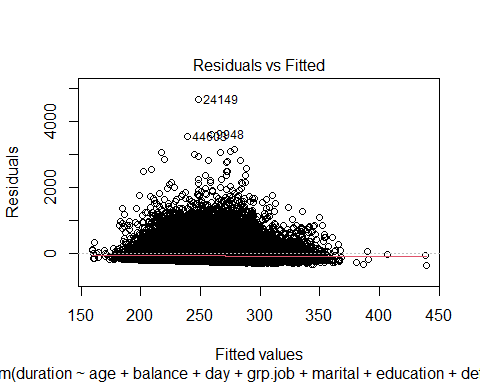
\includegraphics{Bank_files/figure-latex/unnamed-chunk-19-1.pdf}
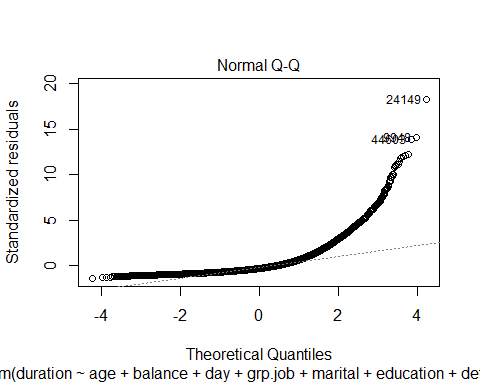
\includegraphics{Bank_files/figure-latex/unnamed-chunk-19-2.pdf}
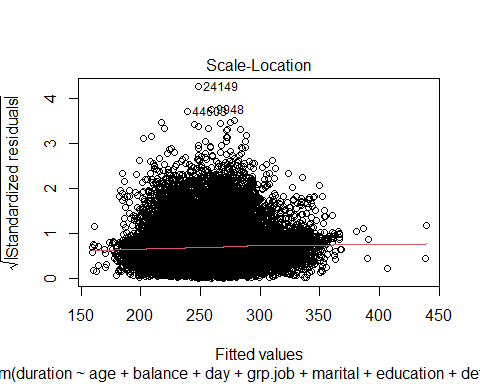
\includegraphics{Bank_files/figure-latex/unnamed-chunk-19-3.pdf}
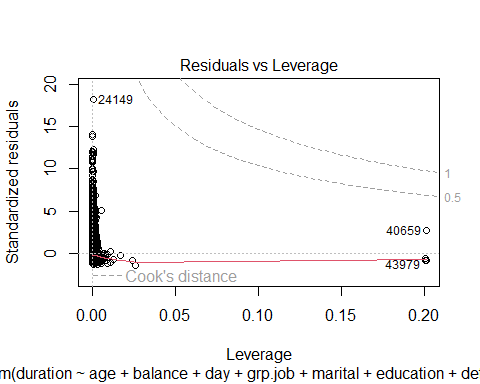
\includegraphics{Bank_files/figure-latex/unnamed-chunk-19-4.pdf}

\begin{Shaded}
\begin{Highlighting}[]
\NormalTok{coefficient.table }\OtherTok{=} \FunctionTok{summary}\NormalTok{(initial.model)}\SpecialCharTok{$}\NormalTok{coef}
\FunctionTok{kable}\NormalTok{(coefficient.table, }\AttributeTok{caption =} \StringTok{"Significance tests of logistic regression model"}\NormalTok{)}
\end{Highlighting}
\end{Shaded}

\begin{longtable}[]{@{}
  >{\raggedright\arraybackslash}p{(\columnwidth - 8\tabcolsep) * \real{0.2029}}
  >{\raggedleft\arraybackslash}p{(\columnwidth - 8\tabcolsep) * \real{0.1884}}
  >{\raggedleft\arraybackslash}p{(\columnwidth - 8\tabcolsep) * \real{0.1739}}
  >{\raggedleft\arraybackslash}p{(\columnwidth - 8\tabcolsep) * \real{0.1594}}
  >{\raggedleft\arraybackslash}p{(\columnwidth - 8\tabcolsep) * \real{0.2754}}@{}}
\caption{Significance tests of logistic regression model}\tabularnewline
\toprule\noalign{}
\begin{minipage}[b]{\linewidth}\raggedright
\end{minipage} & \begin{minipage}[b]{\linewidth}\raggedleft
Estimate
\end{minipage} & \begin{minipage}[b]{\linewidth}\raggedleft
Std. Error
\end{minipage} & \begin{minipage}[b]{\linewidth}\raggedleft
t value
\end{minipage} & \begin{minipage}[b]{\linewidth}\raggedleft
Pr(\textgreater\textbar t\textbar)
\end{minipage} \\
\midrule\noalign{}
\endfirsthead
\toprule\noalign{}
\begin{minipage}[b]{\linewidth}\raggedright
\end{minipage} & \begin{minipage}[b]{\linewidth}\raggedleft
Estimate
\end{minipage} & \begin{minipage}[b]{\linewidth}\raggedleft
Std. Error
\end{minipage} & \begin{minipage}[b]{\linewidth}\raggedleft
t value
\end{minipage} & \begin{minipage}[b]{\linewidth}\raggedleft
Pr(\textgreater\textbar t\textbar)
\end{minipage} \\
\midrule\noalign{}
\endhead
\bottomrule\noalign{}
\endlastfoot
(Intercept) & 278.1019715 & 11.3974233 & 24.4004249 & 0.0000000 \\
age & 0.0083785 & 0.1400149 & 0.0598403 & 0.9522831 \\
balance & 0.0016194 & 0.0004136 & 3.9150836 & 0.0000905 \\
day & -0.7807526 & 0.1506568 & -5.1823251 & 0.0000002 \\
grp.job1 & -11.0742342 & 4.8736308 & -2.2722760 & 0.0230747 \\
grp.job2 & -21.2324631 & 4.9945461 & -4.2511297 & 0.0000213 \\
grp.job3 & -25.5521708 & 4.5833783 & -5.5749644 & 0.0000000 \\
marital1 & 2.4519149 & 4.6382482 & 0.5286295 & 0.5970652 \\
marital2 & -10.6850180 & 4.0030828 & -2.6691974 & 0.0076061 \\
education1 & -3.0816026 & 6.9654635 & -0.4424117 & 0.6581935 \\
education2 & 3.0902802 & 6.3912414 & 0.4835180 & 0.6287304 \\
education3 & 0.8134778 & 6.7958463 & 0.1197022 & 0.9047196 \\
default1 & -16.8459618 & 9.2242703 & -1.8262650 & 0.0678172 \\
housing1 & 11.3060522 & 2.6986059 & 4.1895900 & 0.0000280 \\
loan1 & -4.0230166 & 3.4012535 & -1.1828041 & 0.2368933 \\
contact1 & -8.9728967 & 5.5933888 & -1.6041968 & 0.1086780 \\
contact2 & 15.5759868 & 2.9591009 & 5.2637565 & 0.0000001 \\
grp.campaign1 & 14.4395410 & 2.7973165 & 5.1619261 & 0.0000002 \\
grp.campaign2 & -30.5705356 & 3.4047983 & -8.9786627 & 0.0000000 \\
grp.pdays1 & 89.7478592 & 114.9371431 & 0.7808430 & 0.4348991 \\
grp.pdays2 & 92.0183672 & 114.9937921 & 0.8002029 & 0.4235976 \\
grp.previous1 & -8.1042460 & 8.6448724 & -0.9374628 & 0.3485258 \\
poutcome1 & -36.2983161 & 114.9997510 & -0.3156382 & 0.7522786 \\
poutcome2 & -110.1359174 & 114.8666385 & -0.9588155 & 0.3376570 \\
\end{longtable}

We can see that there are some insignificant predictor variables, and
they should be dropped from the model to create a reduced model. Using
the step() function, we will now find reduced and final models. The
final best model will be a model that is between the full and reduced
models.

\begin{Shaded}
\begin{Highlighting}[]
\FunctionTok{library}\NormalTok{(MASS)}
\FunctionTok{boxcox}\NormalTok{(duration }\SpecialCharTok{\textasciitilde{}}\NormalTok{ age }\SpecialCharTok{+}\NormalTok{ balance }\SpecialCharTok{+}\NormalTok{ day }\SpecialCharTok{+}\NormalTok{ grp.job }\SpecialCharTok{+}\NormalTok{ marital }\SpecialCharTok{+}\NormalTok{ education }\SpecialCharTok{+}\NormalTok{ default }\SpecialCharTok{+}\NormalTok{ housing }\SpecialCharTok{+}\NormalTok{ loan }\SpecialCharTok{+}\NormalTok{ contact }\SpecialCharTok{+}\NormalTok{ grp.campaign}\SpecialCharTok{+}\NormalTok{grp.pdays}\SpecialCharTok{+}\NormalTok{grp.previous}\SpecialCharTok{+}\NormalTok{poutcome, }
       \AttributeTok{data =}\NormalTok{ BankMarketingL, }
       \AttributeTok{lambda =} \FunctionTok{seq}\NormalTok{(}\SpecialCharTok{{-}}\DecValTok{1}\NormalTok{, }\FloatTok{1.5}\NormalTok{, }\AttributeTok{length =} \DecValTok{10}\NormalTok{), }
       \AttributeTok{xlab=}\FunctionTok{expression}\NormalTok{(}\FunctionTok{paste}\NormalTok{(lambda)))}
\FunctionTok{title}\NormalTok{(}\AttributeTok{main =} \StringTok{"Box{-}Cox Transformation: 95\% CI of lambda"}\NormalTok{,}
      \AttributeTok{col.main =} \StringTok{"navy"}\NormalTok{, }\AttributeTok{cex.main =} \FloatTok{0.9}\NormalTok{)}
\end{Highlighting}
\end{Shaded}

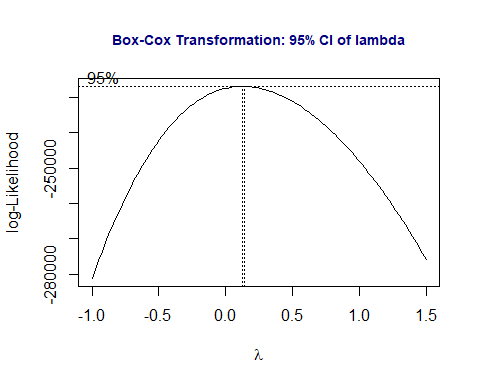
\includegraphics{Bank_files/figure-latex/unnamed-chunk-20-1.pdf}

\begin{Shaded}
\begin{Highlighting}[]
\NormalTok{transform.model }\OtherTok{=} \FunctionTok{lm}\NormalTok{(}\FunctionTok{log}\NormalTok{(duration) }\SpecialCharTok{\textasciitilde{}}\NormalTok{ age }\SpecialCharTok{+}\NormalTok{ balance }\SpecialCharTok{+}\NormalTok{ day }\SpecialCharTok{+}\NormalTok{ grp.job }\SpecialCharTok{+}\NormalTok{ marital }\SpecialCharTok{+}\NormalTok{ education }\SpecialCharTok{+}\NormalTok{ default }\SpecialCharTok{+}\NormalTok{ housing }\SpecialCharTok{+}\NormalTok{ loan }\SpecialCharTok{+}\NormalTok{ contact }\SpecialCharTok{+}\NormalTok{ grp.campaign}\SpecialCharTok{+}\NormalTok{grp.pdays}\SpecialCharTok{+}\NormalTok{grp.previous}\SpecialCharTok{+}\NormalTok{poutcome, }\AttributeTok{data  =}\NormalTok{ BankMarketingL)}
\FunctionTok{par}\NormalTok{(}\AttributeTok{mfrow=}\FunctionTok{c}\NormalTok{(}\DecValTok{2}\NormalTok{,}\DecValTok{2}\NormalTok{), }\AttributeTok{mar =} \FunctionTok{c}\NormalTok{(}\DecValTok{2}\NormalTok{,}\DecValTok{2}\NormalTok{,}\DecValTok{2}\NormalTok{,}\DecValTok{2}\NormalTok{))}
\FunctionTok{plot}\NormalTok{(transform.model)}
\end{Highlighting}
\end{Shaded}

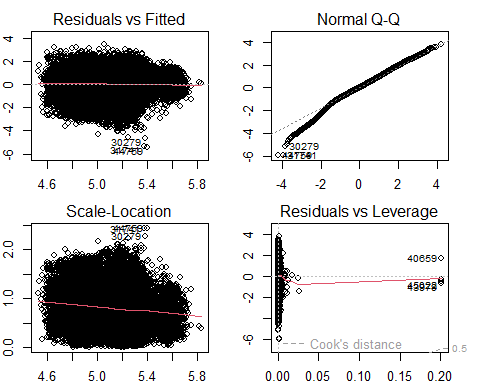
\includegraphics{Bank_files/figure-latex/unnamed-chunk-20-2.pdf}

\begin{Shaded}
\begin{Highlighting}[]
\FunctionTok{kable}\NormalTok{(}\FunctionTok{summary}\NormalTok{(transform.model)}\SpecialCharTok{$}\NormalTok{coef, }\AttributeTok{caption =} \StringTok{"Summarized statistics of the regression }
\StringTok{      coefficients of the model with a log{-}transformed response"}\NormalTok{)}
\end{Highlighting}
\end{Shaded}

\begin{longtable}[]{@{}
  >{\raggedright\arraybackslash}p{(\columnwidth - 8\tabcolsep) * \real{0.2090}}
  >{\raggedleft\arraybackslash}p{(\columnwidth - 8\tabcolsep) * \real{0.1642}}
  >{\raggedleft\arraybackslash}p{(\columnwidth - 8\tabcolsep) * \real{0.1642}}
  >{\raggedleft\arraybackslash}p{(\columnwidth - 8\tabcolsep) * \real{0.1791}}
  >{\raggedleft\arraybackslash}p{(\columnwidth - 8\tabcolsep) * \real{0.2836}}@{}}
\caption{Summarized statistics of the regression coefficients of the
model with a log-transformed response}\tabularnewline
\toprule\noalign{}
\begin{minipage}[b]{\linewidth}\raggedright
\end{minipage} & \begin{minipage}[b]{\linewidth}\raggedleft
Estimate
\end{minipage} & \begin{minipage}[b]{\linewidth}\raggedleft
Std. Error
\end{minipage} & \begin{minipage}[b]{\linewidth}\raggedleft
t value
\end{minipage} & \begin{minipage}[b]{\linewidth}\raggedleft
Pr(\textgreater\textbar t\textbar)
\end{minipage} \\
\midrule\noalign{}
\endfirsthead
\toprule\noalign{}
\begin{minipage}[b]{\linewidth}\raggedright
\end{minipage} & \begin{minipage}[b]{\linewidth}\raggedleft
Estimate
\end{minipage} & \begin{minipage}[b]{\linewidth}\raggedleft
Std. Error
\end{minipage} & \begin{minipage}[b]{\linewidth}\raggedleft
t value
\end{minipage} & \begin{minipage}[b]{\linewidth}\raggedleft
Pr(\textgreater\textbar t\textbar)
\end{minipage} \\
\midrule\noalign{}
\endhead
\bottomrule\noalign{}
\endlastfoot
(Intercept) & 5.2446258 & 0.0404001 & 129.8171789 & 0.0000000 \\
age & 0.0003610 & 0.0004963 & 0.7273715 & 0.4670023 \\
balance & 0.0000046 & 0.0000015 & 3.1105647 & 0.0018685 \\
day & -0.0046024 & 0.0005340 & -8.6183358 & 0.0000000 \\
grp.job1 & -0.0546546 & 0.0172754 & -3.1637207 & 0.0015587 \\
grp.job2 & -0.0809790 & 0.0177040 & -4.5740453 & 0.0000048 \\
grp.job3 & -0.0945196 & 0.0162466 & -5.8178233 & 0.0000000 \\
marital1 & 0.0066519 & 0.0164411 & 0.4045879 & 0.6857825 \\
marital2 & -0.0155715 & 0.0141896 & -1.0973904 & 0.2724769 \\
education1 & 0.0010528 & 0.0246903 & 0.0426405 & 0.9659883 \\
education2 & 0.0353853 & 0.0226548 & 1.5619326 & 0.1183112 \\
education3 & 0.0072181 & 0.0240890 & 0.2996424 & 0.7644514 \\
default1 & -0.0390313 & 0.0326970 & -1.1937290 & 0.2325905 \\
housing1 & 0.0370216 & 0.0095657 & 3.8702601 & 0.0001089 \\
loan1 & -0.0091656 & 0.0120563 & -0.7602324 & 0.4471198 \\
contact1 & -0.1259604 & 0.0198267 & -6.3530670 & 0.0000000 \\
contact2 & 0.1005060 & 0.0104890 & 9.5820066 & 0.0000000 \\
grp.campaign1 & 0.0534748 & 0.0099156 & 5.3930224 & 0.0000001 \\
grp.campaign2 & -0.3061935 & 0.0120689 & -25.3704911 & 0.0000000 \\
grp.pdays1 & 0.3727512 & 0.4074141 & 0.9149197 & 0.3602389 \\
grp.pdays2 & 0.3298483 & 0.4076149 & 0.8092154 & 0.4183957 \\
grp.previous1 & 0.0334652 & 0.0306432 & 1.0920923 & 0.2747986 \\
poutcome1 & -0.1099400 & 0.4076360 & -0.2697013 & 0.7873914 \\
poutcome2 & -0.4576910 & 0.4071642 & -1.1240945 & 0.2609792 \\
\end{longtable}

\begin{Shaded}
\begin{Highlighting}[]
\DocumentationTok{\#\#}
\NormalTok{final.model }\OtherTok{=}  \FunctionTok{step}\NormalTok{(transform.model, }\AttributeTok{direction =} \StringTok{"backward"}\NormalTok{, }\AttributeTok{trace =} \DecValTok{0}\NormalTok{)}
\FunctionTok{kable}\NormalTok{(}\FunctionTok{summary}\NormalTok{(final.model)}\SpecialCharTok{$}\NormalTok{coef, }\AttributeTok{caption =} \StringTok{"Summary statistics of the regression }
\StringTok{      coefficients of the final model"}\NormalTok{)}
\end{Highlighting}
\end{Shaded}

\begin{longtable}[]{@{}
  >{\raggedright\arraybackslash}p{(\columnwidth - 8\tabcolsep) * \real{0.2090}}
  >{\raggedleft\arraybackslash}p{(\columnwidth - 8\tabcolsep) * \real{0.1642}}
  >{\raggedleft\arraybackslash}p{(\columnwidth - 8\tabcolsep) * \real{0.1642}}
  >{\raggedleft\arraybackslash}p{(\columnwidth - 8\tabcolsep) * \real{0.1791}}
  >{\raggedleft\arraybackslash}p{(\columnwidth - 8\tabcolsep) * \real{0.2836}}@{}}
\caption{Summary statistics of the regression coefficients of the final
model}\tabularnewline
\toprule\noalign{}
\begin{minipage}[b]{\linewidth}\raggedright
\end{minipage} & \begin{minipage}[b]{\linewidth}\raggedleft
Estimate
\end{minipage} & \begin{minipage}[b]{\linewidth}\raggedleft
Std. Error
\end{minipage} & \begin{minipage}[b]{\linewidth}\raggedleft
t value
\end{minipage} & \begin{minipage}[b]{\linewidth}\raggedleft
Pr(\textgreater\textbar t\textbar)
\end{minipage} \\
\midrule\noalign{}
\endfirsthead
\toprule\noalign{}
\begin{minipage}[b]{\linewidth}\raggedright
\end{minipage} & \begin{minipage}[b]{\linewidth}\raggedleft
Estimate
\end{minipage} & \begin{minipage}[b]{\linewidth}\raggedleft
Std. Error
\end{minipage} & \begin{minipage}[b]{\linewidth}\raggedleft
t value
\end{minipage} & \begin{minipage}[b]{\linewidth}\raggedleft
Pr(\textgreater\textbar t\textbar)
\end{minipage} \\
\midrule\noalign{}
\endhead
\bottomrule\noalign{}
\endlastfoot
(Intercept) & 5.2568691 & 0.0270577 & 194.2834143 & 0.0000000 \\
balance & 0.0000049 & 0.0000015 & 3.3433635 & 0.0008284 \\
day & -0.0045638 & 0.0005332 & -8.5599667 & 0.0000000 \\
grp.job1 & -0.0608151 & 0.0168262 & -3.6143003 & 0.0003015 \\
grp.job2 & -0.0863436 & 0.0174652 & -4.9437415 & 0.0000008 \\
grp.job3 & -0.0981317 & 0.0158954 & -6.1735990 & 0.0000000 \\
education1 & -0.0015857 & 0.0246293 & -0.0643814 & 0.9486669 \\
education2 & 0.0336210 & 0.0225818 & 1.4888525 & 0.1365335 \\
education3 & 0.0085905 & 0.0239801 & 0.3582348 & 0.7201693 \\
housing1 & 0.0341156 & 0.0093986 & 3.6298434 & 0.0002839 \\
contact1 & -0.1263981 & 0.0196831 & -6.4216538 & 0.0000000 \\
contact2 & 0.0996263 & 0.0104714 & 9.5141151 & 0.0000000 \\
grp.campaign1 & 0.0522764 & 0.0099031 & 5.2788041 & 0.0000001 \\
grp.campaign2 & -0.3083250 & 0.0120384 & -25.6117119 & 0.0000000 \\
poutcome1 & 0.2836532 & 0.0243289 & 11.6591264 & 0.0000000 \\
poutcome2 & -0.0791844 & 0.0145742 & -5.4332078 & 0.0000001 \\
\end{longtable}

\subsection{Use Cross-validation for Model
Selection}\label{use-cross-validation-for-model-selection}

Use cross-validation and MSE as a predictive performance measure to
select the best model.

Now we have three candidate models to select from. We extract the
coefficient of determination R2 of each of the three candidate models.

\begin{Shaded}
\begin{Highlighting}[]
\NormalTok{r.ini.model }\OtherTok{=} \FunctionTok{summary}\NormalTok{(initial.model)}\SpecialCharTok{$}\NormalTok{r.squared}
\NormalTok{r.transfd.model }\OtherTok{=} \FunctionTok{summary}\NormalTok{(transform.model)}\SpecialCharTok{$}\NormalTok{r.squared}
\NormalTok{r.final.model }\OtherTok{=} \FunctionTok{summary}\NormalTok{(final.model)}\SpecialCharTok{$}\NormalTok{r.squared}
\DocumentationTok{\#\#}
\NormalTok{Rsquare }\OtherTok{=} \FunctionTok{cbind}\NormalTok{(}\AttributeTok{initial.model =}\NormalTok{ r.ini.model, }\AttributeTok{transfd.model =}\NormalTok{ r.transfd.model, }
                \AttributeTok{final.model =}\NormalTok{ r.final.model)}
\FunctionTok{kable}\NormalTok{(Rsquare, }\AttributeTok{caption=}\StringTok{"Coefficients of correlation of the three candidate models"}\NormalTok{)}
\end{Highlighting}
\end{Shaded}

\begin{longtable}[]{@{}rrr@{}}
\caption{Coefficients of correlation of the three candidate
models}\tabularnewline
\toprule\noalign{}
initial.model & transfd.model & final.model \\
\midrule\noalign{}
\endfirsthead
\toprule\noalign{}
initial.model & transfd.model & final.model \\
\midrule\noalign{}
\endhead
\bottomrule\noalign{}
\endlastfoot
0.0106387 & 0.0376558 & 0.0373992 \\
\end{longtable}

All three of these models are frankly terrible with Rsquare scores of
1.1, 3.76 and 3.37. Out of the three the best performing model is the
reduced/transformed model. The summary of the transformed model is seen
below.

\begin{Shaded}
\begin{Highlighting}[]
\FunctionTok{kable}\NormalTok{(}\FunctionTok{summary}\NormalTok{(transform.model)}\SpecialCharTok{$}\NormalTok{coef, }\AttributeTok{caption =} \StringTok{"Summarized statistics of the regression }
\StringTok{      coefficients of the model with a log{-}transformed response"}\NormalTok{)}
\end{Highlighting}
\end{Shaded}

\begin{longtable}[]{@{}
  >{\raggedright\arraybackslash}p{(\columnwidth - 8\tabcolsep) * \real{0.2090}}
  >{\raggedleft\arraybackslash}p{(\columnwidth - 8\tabcolsep) * \real{0.1642}}
  >{\raggedleft\arraybackslash}p{(\columnwidth - 8\tabcolsep) * \real{0.1642}}
  >{\raggedleft\arraybackslash}p{(\columnwidth - 8\tabcolsep) * \real{0.1791}}
  >{\raggedleft\arraybackslash}p{(\columnwidth - 8\tabcolsep) * \real{0.2836}}@{}}
\caption{Summarized statistics of the regression coefficients of the
model with a log-transformed response}\tabularnewline
\toprule\noalign{}
\begin{minipage}[b]{\linewidth}\raggedright
\end{minipage} & \begin{minipage}[b]{\linewidth}\raggedleft
Estimate
\end{minipage} & \begin{minipage}[b]{\linewidth}\raggedleft
Std. Error
\end{minipage} & \begin{minipage}[b]{\linewidth}\raggedleft
t value
\end{minipage} & \begin{minipage}[b]{\linewidth}\raggedleft
Pr(\textgreater\textbar t\textbar)
\end{minipage} \\
\midrule\noalign{}
\endfirsthead
\toprule\noalign{}
\begin{minipage}[b]{\linewidth}\raggedright
\end{minipage} & \begin{minipage}[b]{\linewidth}\raggedleft
Estimate
\end{minipage} & \begin{minipage}[b]{\linewidth}\raggedleft
Std. Error
\end{minipage} & \begin{minipage}[b]{\linewidth}\raggedleft
t value
\end{minipage} & \begin{minipage}[b]{\linewidth}\raggedleft
Pr(\textgreater\textbar t\textbar)
\end{minipage} \\
\midrule\noalign{}
\endhead
\bottomrule\noalign{}
\endlastfoot
(Intercept) & 5.2446258 & 0.0404001 & 129.8171789 & 0.0000000 \\
age & 0.0003610 & 0.0004963 & 0.7273715 & 0.4670023 \\
balance & 0.0000046 & 0.0000015 & 3.1105647 & 0.0018685 \\
day & -0.0046024 & 0.0005340 & -8.6183358 & 0.0000000 \\
grp.job1 & -0.0546546 & 0.0172754 & -3.1637207 & 0.0015587 \\
grp.job2 & -0.0809790 & 0.0177040 & -4.5740453 & 0.0000048 \\
grp.job3 & -0.0945196 & 0.0162466 & -5.8178233 & 0.0000000 \\
marital1 & 0.0066519 & 0.0164411 & 0.4045879 & 0.6857825 \\
marital2 & -0.0155715 & 0.0141896 & -1.0973904 & 0.2724769 \\
education1 & 0.0010528 & 0.0246903 & 0.0426405 & 0.9659883 \\
education2 & 0.0353853 & 0.0226548 & 1.5619326 & 0.1183112 \\
education3 & 0.0072181 & 0.0240890 & 0.2996424 & 0.7644514 \\
default1 & -0.0390313 & 0.0326970 & -1.1937290 & 0.2325905 \\
housing1 & 0.0370216 & 0.0095657 & 3.8702601 & 0.0001089 \\
loan1 & -0.0091656 & 0.0120563 & -0.7602324 & 0.4471198 \\
contact1 & -0.1259604 & 0.0198267 & -6.3530670 & 0.0000000 \\
contact2 & 0.1005060 & 0.0104890 & 9.5820066 & 0.0000000 \\
grp.campaign1 & 0.0534748 & 0.0099156 & 5.3930224 & 0.0000001 \\
grp.campaign2 & -0.3061935 & 0.0120689 & -25.3704911 & 0.0000000 \\
grp.pdays1 & 0.3727512 & 0.4074141 & 0.9149197 & 0.3602389 \\
grp.pdays2 & 0.3298483 & 0.4076149 & 0.8092154 & 0.4183957 \\
grp.previous1 & 0.0334652 & 0.0306432 & 1.0920923 & 0.2747986 \\
poutcome1 & -0.1099400 & 0.4076360 & -0.2697013 & 0.7873914 \\
poutcome2 & -0.4576910 & 0.4071642 & -1.1240945 & 0.2609792 \\
\end{longtable}

\subsection{Results and Conclusions}\label{results-and-conclusions}

Report results based on the final model and conclude the statement of
questions.

In summary, balance, day, job, housing, contact, and campaign are
statistically significant (p-value \textless.05). Day and job negatively
correlated to duration. Balance, housing, contact and campaign are
positively correlated. When given a the balance of an account (balance)
and increases by 1 , and all other variables are held constant, there is
an 0.0000046 second increase in duration. Alternatively, when given the
day and it changes to the next, and all other variables are held
constant, there is a 0.0046024 second decrease in the duration of a
call.

\section{Logistic Regression}\label{logistic-regression}

We can use a logistical model for predicting whether or not a client has
subscribed a term deposit after direct marketing campaigns.The variable,
y, which tells whether a client has subscribed a term deposit, acts as
the binary response variable of all the logistic models. The rest of the
variables, including the new discretized variables, of the revised data
set act as the predictor variables that will possibly affect the
response `y'.

\subsection{Create Candidate Models}\label{create-candidate-models-1}

The full/initial model containing all of the predictor variables will be
made first, with `y' (whether or not a client has subscribed a term
deposit) as the response. The variables balance and default are not
included since our EDA showed that removing them from the model might
help the results.

\begin{Shaded}
\begin{Highlighting}[]
\CommentTok{\# Create the initial full model}
\NormalTok{initial.model }\OtherTok{=} \FunctionTok{glm}\NormalTok{(y }\SpecialCharTok{\textasciitilde{}}\NormalTok{ age }\SpecialCharTok{+}\NormalTok{ day }\SpecialCharTok{+}\NormalTok{ grp.job }\SpecialCharTok{+}\NormalTok{ marital }\SpecialCharTok{+}\NormalTok{ education }\SpecialCharTok{+}\NormalTok{ housing }\SpecialCharTok{+}\NormalTok{ loan }\SpecialCharTok{+}\NormalTok{ contact }\SpecialCharTok{+}\NormalTok{ grp.duration }\SpecialCharTok{+}\NormalTok{ grp.campaign }\SpecialCharTok{+}\NormalTok{ grp.pdays }\SpecialCharTok{+}\NormalTok{ grp.previous, }\AttributeTok{family =}\NormalTok{ binomial, }\AttributeTok{data =}\NormalTok{ BankMarketingCampaign)}
\NormalTok{coefficient.table }\OtherTok{=} \FunctionTok{summary}\NormalTok{(initial.model)}\SpecialCharTok{$}\NormalTok{coef}
\FunctionTok{kable}\NormalTok{(coefficient.table, }\AttributeTok{caption =} \StringTok{"Significance tests of logistic regression model"}\NormalTok{)}
\end{Highlighting}
\end{Shaded}

\begin{longtable}[]{@{}lrrrr@{}}
\caption{Significance tests of logistic regression model}\tabularnewline
\toprule\noalign{}
& Estimate & Std. Error & z value &
Pr(\textgreater\textbar z\textbar) \\
\midrule\noalign{}
\endfirsthead
\toprule\noalign{}
& Estimate & Std. Error & z value &
Pr(\textgreater\textbar z\textbar) \\
\midrule\noalign{}
\endhead
\bottomrule\noalign{}
\endlastfoot
(Intercept) & -3.5018560 & 0.1521815 & -23.011052 & 0.0000000 \\
age & 0.0037427 & 0.0017733 & 2.110553 & 0.0348108 \\
day & -0.0055270 & 0.0020224 & -2.732896 & 0.0062780 \\
grp.job1 & -0.5356687 & 0.0623519 & -8.591057 & 0.0000000 \\
grp.job2 & -0.4527472 & 0.0599608 & -7.550719 & 0.0000000 \\
grp.job3 & -0.3669178 & 0.0546304 & -6.716368 & 0.0000000 \\
marital1 & 0.1692006 & 0.0610871 & 2.769826 & 0.0056086 \\
marital2 & -0.1806493 & 0.0536963 & -3.364279 & 0.0007674 \\
education1 & -0.2609743 & 0.0938475 & -2.780833 & 0.0054220 \\
education2 & -0.1221068 & 0.0829586 & -1.471899 & 0.1410481 \\
education3 & 0.1775338 & 0.0866458 & 2.048960 & 0.0404660 \\
housing1 & -0.7303848 & 0.0366351 & -19.936773 & 0.0000000 \\
loan1 & -0.5591949 & 0.0540381 & -10.348154 & 0.0000000 \\
contact1 & 0.9550897 & 0.0817113 & 11.688589 & 0.0000000 \\
contact2 & 1.0053064 & 0.0523061 & 19.219696 & 0.0000000 \\
grp.duration1 & 1.3339942 & 0.0503148 & 26.512978 & 0.0000000 \\
grp.duration2 & 2.7044986 & 0.0458332 & 59.007422 & 0.0000000 \\
grp.campaign1 & -0.3253327 & 0.0364818 & -8.917665 & 0.0000000 \\
grp.campaign2 & -0.5201170 & 0.0505253 & -10.294181 & 0.0000000 \\
grp.pdays1 & 1.4641585 & 0.0758033 & 19.315236 & 0.0000000 \\
grp.pdays2 & 0.6043423 & 0.0869219 & 6.952701 & 0.0000000 \\
grp.previous1 & -0.2153398 & 0.0777604 & -2.769273 & 0.0056181 \\
\end{longtable}

We can see that there are some insignificant predictor variables, and
they should be dropped from the model to create a reduced model. Using
the step() function, we will now find reduced and final models. The
final best model will be a model that is between the full and reduced
models.

\begin{Shaded}
\begin{Highlighting}[]
\CommentTok{\# Creating the reduced and final models}
\NormalTok{full.model }\OtherTok{=}\NormalTok{ initial.model  }\CommentTok{\# the *biggest model* that includes all predictor variables}
\NormalTok{reduced.model }\OtherTok{=} \FunctionTok{glm}\NormalTok{(y }\SpecialCharTok{\textasciitilde{}}\NormalTok{ day }\SpecialCharTok{+}\NormalTok{ grp.job }\SpecialCharTok{+}\NormalTok{ marital }\SpecialCharTok{+}\NormalTok{ housing }\SpecialCharTok{+}\NormalTok{ loan }\SpecialCharTok{+}\NormalTok{ contact }\SpecialCharTok{+}\NormalTok{ grp.duration }\SpecialCharTok{+}\NormalTok{ grp.campaign }\SpecialCharTok{+}\NormalTok{ grp.previous, }\AttributeTok{family =}\NormalTok{ binomial, }\AttributeTok{data =}\NormalTok{ BankMarketingCampaign)}
\NormalTok{final.model }\OtherTok{=}  \FunctionTok{step}\NormalTok{(full.model, }
                    \AttributeTok{scope=}\FunctionTok{list}\NormalTok{(}\AttributeTok{lower=}\FunctionTok{formula}\NormalTok{(reduced.model),}\AttributeTok{upper=}\FunctionTok{formula}\NormalTok{(full.model)),}
                    \AttributeTok{data =}\NormalTok{ BankMarketingCampaign, }
                    \AttributeTok{direction =} \StringTok{"backward"}\NormalTok{,}
                    \AttributeTok{trace =} \DecValTok{0}\NormalTok{)   }\CommentTok{\# trace = 0: suppress the detailed selection process}
\NormalTok{final.model.coef }\OtherTok{=} \FunctionTok{summary}\NormalTok{(final.model)}\SpecialCharTok{$}\NormalTok{coef}
\FunctionTok{kable}\NormalTok{(final.model.coef, }\AttributeTok{caption =} \StringTok{"Summary table of significant tests"}\NormalTok{)}
\end{Highlighting}
\end{Shaded}

\begin{longtable}[]{@{}lrrrr@{}}
\caption{Summary table of significant tests}\tabularnewline
\toprule\noalign{}
& Estimate & Std. Error & z value &
Pr(\textgreater\textbar z\textbar) \\
\midrule\noalign{}
\endfirsthead
\toprule\noalign{}
& Estimate & Std. Error & z value &
Pr(\textgreater\textbar z\textbar) \\
\midrule\noalign{}
\endhead
\bottomrule\noalign{}
\endlastfoot
(Intercept) & -3.5018560 & 0.1521815 & -23.011052 & 0.0000000 \\
age & 0.0037427 & 0.0017733 & 2.110553 & 0.0348108 \\
day & -0.0055270 & 0.0020224 & -2.732896 & 0.0062780 \\
grp.job1 & -0.5356687 & 0.0623519 & -8.591057 & 0.0000000 \\
grp.job2 & -0.4527472 & 0.0599608 & -7.550719 & 0.0000000 \\
grp.job3 & -0.3669178 & 0.0546304 & -6.716368 & 0.0000000 \\
marital1 & 0.1692006 & 0.0610871 & 2.769826 & 0.0056086 \\
marital2 & -0.1806493 & 0.0536963 & -3.364279 & 0.0007674 \\
education1 & -0.2609743 & 0.0938475 & -2.780833 & 0.0054220 \\
education2 & -0.1221068 & 0.0829586 & -1.471899 & 0.1410481 \\
education3 & 0.1775338 & 0.0866458 & 2.048960 & 0.0404660 \\
housing1 & -0.7303848 & 0.0366351 & -19.936773 & 0.0000000 \\
loan1 & -0.5591949 & 0.0540381 & -10.348154 & 0.0000000 \\
contact1 & 0.9550897 & 0.0817113 & 11.688589 & 0.0000000 \\
contact2 & 1.0053064 & 0.0523061 & 19.219696 & 0.0000000 \\
grp.duration1 & 1.3339942 & 0.0503148 & 26.512978 & 0.0000000 \\
grp.duration2 & 2.7044986 & 0.0458332 & 59.007422 & 0.0000000 \\
grp.campaign1 & -0.3253327 & 0.0364818 & -8.917665 & 0.0000000 \\
grp.campaign2 & -0.5201170 & 0.0505253 & -10.294181 & 0.0000000 \\
grp.pdays1 & 1.4641585 & 0.0758033 & 19.315236 & 0.0000000 \\
grp.pdays2 & 0.6043423 & 0.0869219 & 6.952701 & 0.0000000 \\
grp.previous1 & -0.2153398 & 0.0777604 & -2.769273 & 0.0056181 \\
\end{longtable}

\subsection{Model Selection}\label{model-selection}

Now that we have our canidate models. It is time to perform some model
selction using the ROC curve and AUC.

Since our sample is relatively large, we will randomly split the overall
data set into two data sets. 70\% of the data will be put in a training
data set for training and validating models. The other 30\% goes into a
testing data set used for testing the final model. The value labels of
the response (yes/no) used for testing and validation data will be
removed when calculating the accuracy measures later.

\begin{Shaded}
\begin{Highlighting}[]
\DocumentationTok{\#\# Recode response variable: yes = 1 and no = 0}
\NormalTok{yes.id }\OtherTok{=} \FunctionTok{which}\NormalTok{(BankMarketingCampaign}\SpecialCharTok{$}\NormalTok{y }\SpecialCharTok{==} \StringTok{"1"}\NormalTok{) }
\NormalTok{no.id }\OtherTok{=} \FunctionTok{which}\NormalTok{(BankMarketingCampaign}\SpecialCharTok{$}\NormalTok{y }\SpecialCharTok{==} \StringTok{"0"}\NormalTok{)}

\DocumentationTok{\#\# Creating the training and testing data sets}
\NormalTok{BankMarketingCampaign}\SpecialCharTok{$}\NormalTok{y.subscribe }\OtherTok{=} \DecValTok{1}
\NormalTok{BankMarketingCampaign}\SpecialCharTok{$}\NormalTok{y.subscribe[no.id] }\OtherTok{=} \DecValTok{0}
\NormalTok{var.names }\OtherTok{=} \FunctionTok{c}\NormalTok{(}\StringTok{"age"}\NormalTok{, }\StringTok{"day"}\NormalTok{, }\StringTok{"grp.job"}\NormalTok{, }\StringTok{"marital"}\NormalTok{,}\StringTok{"education"}\NormalTok{,}\StringTok{"housing"}\NormalTok{,}\StringTok{"loan"}\NormalTok{,}\StringTok{"contact"}\NormalTok{,}\StringTok{"grp.month"}\NormalTok{,    }\StringTok{"grp.duration"}\NormalTok{,}\StringTok{"grp.campaign"}\NormalTok{,}\StringTok{"grp.pdays"}\NormalTok{,}\StringTok{"grp.previous"}\NormalTok{, }\StringTok{"y.subscribe"}\NormalTok{ )}
\NormalTok{BankMarketingCampaign }\OtherTok{=}\NormalTok{ BankMarketingCampaign[, var.names]}
\NormalTok{nn }\OtherTok{=} \FunctionTok{dim}\NormalTok{(BankMarketingCampaign)[}\DecValTok{1}\NormalTok{]}
\NormalTok{train.id }\OtherTok{=} \FunctionTok{sample}\NormalTok{(}\DecValTok{1}\SpecialCharTok{:}\NormalTok{nn, }\FunctionTok{round}\NormalTok{(nn}\SpecialCharTok{*}\FloatTok{0.7}\NormalTok{), }\AttributeTok{replace =} \ConstantTok{FALSE}\NormalTok{) }
\DocumentationTok{\#\#\#\#}
\NormalTok{training }\OtherTok{=}\NormalTok{ BankMarketingCampaign[train.id,]}
\NormalTok{testing }\OtherTok{=}\NormalTok{ BankMarketingCampaign[}\SpecialCharTok{{-}}\NormalTok{train.id,]}
\end{Highlighting}
\end{Shaded}

\subsection{Cut-off Probability Search and Accuracy
Score}\label{cut-off-probability-search-and-accuracy-score}

In order to find an optimal cut-off probability, a sequence of 20
candidate cut-off probabilities will be defined. Then, a 5-fold
cross-validation will be performed to find the optimal cut-off
probability of the final model. All three models created will be used to
find the optimal cut-off. This is shown below.

\begin{Shaded}
\begin{Highlighting}[]
\NormalTok{n0 }\OtherTok{=} \FunctionTok{dim}\NormalTok{(training)[}\DecValTok{1}\NormalTok{]}\SpecialCharTok{/}\DecValTok{5}

\CommentTok{\# candidate cut off prob}
\NormalTok{cut}\FloatTok{.0}\NormalTok{ff.prob }\OtherTok{=} \FunctionTok{seq}\NormalTok{(}\DecValTok{0}\NormalTok{,}\DecValTok{1}\NormalTok{, }\AttributeTok{length =} \DecValTok{22}\NormalTok{)[}\SpecialCharTok{{-}}\FunctionTok{c}\NormalTok{(}\DecValTok{1}\NormalTok{,}\DecValTok{22}\NormalTok{)]}

\CommentTok{\# null vector for storing prediction accuracy}
\NormalTok{pred.accuracy }\OtherTok{=} \FunctionTok{matrix}\NormalTok{(}\DecValTok{0}\NormalTok{,}\AttributeTok{ncol=}\DecValTok{20}\NormalTok{, }\AttributeTok{nrow=}\DecValTok{5}\NormalTok{, }\AttributeTok{byrow =}\NormalTok{ T)}

\DocumentationTok{\#\# 5{-}fold CV}
\ControlFlowTok{for}\NormalTok{ (i }\ControlFlowTok{in} \DecValTok{1}\SpecialCharTok{:}\DecValTok{5}\NormalTok{)\{}
\NormalTok{  valid.id }\OtherTok{=}\NormalTok{ ((i}\DecValTok{{-}1}\NormalTok{)}\SpecialCharTok{*}\NormalTok{n0 }\SpecialCharTok{+} \DecValTok{1}\NormalTok{)}\SpecialCharTok{:}\NormalTok{(i}\SpecialCharTok{*}\NormalTok{n0)}
\NormalTok{  valid.data }\OtherTok{=}\NormalTok{ training[valid.id,]}
\NormalTok{  train.data }\OtherTok{=}\NormalTok{ training[}\SpecialCharTok{{-}}\NormalTok{valid.id,]}
\NormalTok{  train.model }\OtherTok{=} \FunctionTok{glm}\NormalTok{(y.subscribe }\SpecialCharTok{\textasciitilde{}}\NormalTok{ age }\SpecialCharTok{+}\NormalTok{ day }\SpecialCharTok{+}\NormalTok{ grp.job }\SpecialCharTok{+}\NormalTok{ marital }\SpecialCharTok{+}\NormalTok{ education }\SpecialCharTok{+}\NormalTok{ housing }\SpecialCharTok{+}\NormalTok{ loan }\SpecialCharTok{+}\NormalTok{ contact }\SpecialCharTok{+}\NormalTok{  grp.duration }\SpecialCharTok{+}\NormalTok{ grp.campaign }\SpecialCharTok{+}\NormalTok{ grp.pdays }\SpecialCharTok{+}\NormalTok{ grp.previous, }\AttributeTok{family =} \FunctionTok{binomial}\NormalTok{(}\AttributeTok{link =}\NormalTok{ logit), }\AttributeTok{data =}\NormalTok{ train.data)}
\DocumentationTok{\#\#\#\#}
\NormalTok{  pred.prob }\OtherTok{=} \FunctionTok{predict.glm}\NormalTok{(train.model, valid.data, }\AttributeTok{type =} \StringTok{"response"}\NormalTok{)}
  \CommentTok{\# define confusion matrix and accuracy}
  \ControlFlowTok{for}\NormalTok{(j }\ControlFlowTok{in} \DecValTok{1}\SpecialCharTok{:}\DecValTok{20}\NormalTok{)\{}
    \CommentTok{\#pred.subscribe = rep(0,length(pred.prob))}
\NormalTok{    valid.data}\SpecialCharTok{$}\NormalTok{pred.subscribe }\OtherTok{=} \FunctionTok{as.numeric}\NormalTok{(pred.prob }\SpecialCharTok{\textgreater{}}\NormalTok{ cut}\FloatTok{.0}\NormalTok{ff.prob[j])}
\NormalTok{    a11 }\OtherTok{=} \FunctionTok{sum}\NormalTok{(valid.data}\SpecialCharTok{$}\NormalTok{pred.subscribe }\SpecialCharTok{==}\NormalTok{ valid.data}\SpecialCharTok{$}\NormalTok{y.subscribe)}
\NormalTok{    pred.accuracy[i,j] }\OtherTok{=}\NormalTok{ a11}\SpecialCharTok{/}\FunctionTok{length}\NormalTok{(pred.prob)}
\NormalTok{  \}}
\NormalTok{\}}
\DocumentationTok{\#\#}
\NormalTok{avg.accuracy }\OtherTok{=} \FunctionTok{apply}\NormalTok{(pred.accuracy, }\DecValTok{2}\NormalTok{, mean)}
\NormalTok{max.id }\OtherTok{=} \FunctionTok{which}\NormalTok{(avg.accuracy }\SpecialCharTok{==}\FunctionTok{max}\NormalTok{(avg.accuracy))}

\DocumentationTok{\#\#\# visual representation}
\NormalTok{tick.label }\OtherTok{=} \FunctionTok{as.character}\NormalTok{(}\FunctionTok{round}\NormalTok{(cut}\FloatTok{.0}\NormalTok{ff.prob,}\DecValTok{2}\NormalTok{))}
\FunctionTok{plot}\NormalTok{(}\DecValTok{1}\SpecialCharTok{:}\DecValTok{20}\NormalTok{, avg.accuracy, }\AttributeTok{type =} \StringTok{"b"}\NormalTok{,}
     \AttributeTok{xlim=}\FunctionTok{c}\NormalTok{(}\DecValTok{1}\NormalTok{,}\DecValTok{20}\NormalTok{), }
     \AttributeTok{ylim=}\FunctionTok{c}\NormalTok{(}\FloatTok{0.5}\NormalTok{,}\DecValTok{1}\NormalTok{), }
     \AttributeTok{axes =} \ConstantTok{FALSE}\NormalTok{,}
     \AttributeTok{xlab =} \StringTok{"Cut{-}off Probability"}\NormalTok{,}
     \AttributeTok{ylab =} \StringTok{"Accuracy"}\NormalTok{,}
     \AttributeTok{main =} \StringTok{"5{-}fold CV performance"}
\NormalTok{     )}
\FunctionTok{axis}\NormalTok{(}\DecValTok{1}\NormalTok{, }\AttributeTok{at=}\DecValTok{1}\SpecialCharTok{:}\DecValTok{20}\NormalTok{, }\AttributeTok{label =}\NormalTok{ tick.label, }\AttributeTok{las =} \DecValTok{2}\NormalTok{)}
\FunctionTok{axis}\NormalTok{(}\DecValTok{2}\NormalTok{)}
\FunctionTok{segments}\NormalTok{(max.id, }\FloatTok{0.5}\NormalTok{, max.id, avg.accuracy[max.id], }\AttributeTok{col =} \StringTok{"red"}\NormalTok{)}
\FunctionTok{text}\NormalTok{(max.id, avg.accuracy[max.id]}\SpecialCharTok{+}\FloatTok{0.03}\NormalTok{, }\FunctionTok{as.character}\NormalTok{(}\FunctionTok{round}\NormalTok{(avg.accuracy[max.id],}\DecValTok{4}\NormalTok{)), }\AttributeTok{col =} \StringTok{"red"}\NormalTok{, }\AttributeTok{cex =} \FloatTok{0.8}\NormalTok{)}
\end{Highlighting}
\end{Shaded}

\begin{figure}

{\centering 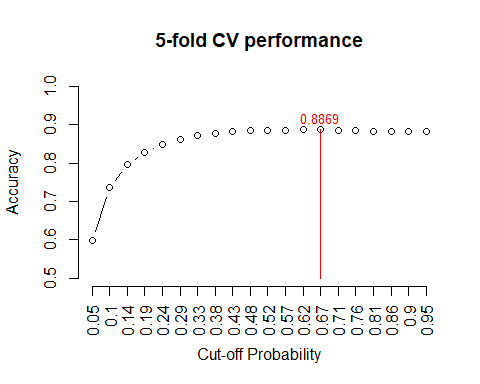
\includegraphics{Bank_files/figure-latex/unnamed-chunk-26-1} 

}

\caption{5-fold CV performance plot}\label{fig:unnamed-chunk-26}
\end{figure}

The above figure indicates that the optimal cut-off probability that
yields the best accuracy is 0.57.

\begin{Shaded}
\begin{Highlighting}[]
\DocumentationTok{\#\# Creation of testing model}
\NormalTok{test.model }\OtherTok{=} \FunctionTok{glm}\NormalTok{(y.subscribe }\SpecialCharTok{\textasciitilde{}}\NormalTok{ age }\SpecialCharTok{+}\NormalTok{ day }\SpecialCharTok{+}\NormalTok{ grp.job }\SpecialCharTok{+}\NormalTok{ marital }\SpecialCharTok{+}\NormalTok{ education }\SpecialCharTok{+}\NormalTok{ housing }\SpecialCharTok{+}\NormalTok{ loan }\SpecialCharTok{+}\NormalTok{ contact }\SpecialCharTok{+}\NormalTok{ grp.duration }\SpecialCharTok{+}\NormalTok{ grp.campaign }\SpecialCharTok{+}\NormalTok{ grp.pdays }\SpecialCharTok{+}\NormalTok{ grp.previous, }\AttributeTok{family =} \FunctionTok{binomial}\NormalTok{(}\AttributeTok{link =}\NormalTok{ logit), }\AttributeTok{data =}\NormalTok{ training)}
\NormalTok{newBankingTestingData }\OtherTok{=} \FunctionTok{data.frame}\NormalTok{(}\AttributeTok{age=}\NormalTok{ testing}\SpecialCharTok{$}\NormalTok{age, }\AttributeTok{day=}\NormalTok{ testing}\SpecialCharTok{$}\NormalTok{day, }\AttributeTok{grp.job=}\NormalTok{ testing}\SpecialCharTok{$}\NormalTok{grp.job, }\AttributeTok{marital=}\NormalTok{ testing}\SpecialCharTok{$}\NormalTok{marital, }\AttributeTok{education=}\NormalTok{ testing}\SpecialCharTok{$}\NormalTok{education, }\AttributeTok{housing=}\NormalTok{ testing}\SpecialCharTok{$}\NormalTok{housing, }\AttributeTok{loan=}\NormalTok{ testing}\SpecialCharTok{$}\NormalTok{loan, }\AttributeTok{contact=}\NormalTok{ testing}\SpecialCharTok{$}\NormalTok{contact, }\AttributeTok{grp.month=}\NormalTok{ testing}\SpecialCharTok{$}\NormalTok{grp.month, }\AttributeTok{grp.duration=}\NormalTok{ testing}\SpecialCharTok{$}\NormalTok{grp.duration, }\AttributeTok{grp.campaign=}\NormalTok{ testing}\SpecialCharTok{$}\NormalTok{grp.campaign, }\AttributeTok{grp.pdays=}\NormalTok{ testing}\SpecialCharTok{$}\NormalTok{grp.pdays, }\AttributeTok{grp.previous=}\NormalTok{ testing}\SpecialCharTok{$}\NormalTok{grp.previous)}

\NormalTok{pred.prob.test }\OtherTok{=} \FunctionTok{predict.glm}\NormalTok{(test.model, newBankingTestingData, }\AttributeTok{type =} \StringTok{"response"}\NormalTok{)}

\DocumentationTok{\#\# Assessing Model Accuracy}
\NormalTok{testing}\SpecialCharTok{$}\NormalTok{test.subscribe }\OtherTok{=} \FunctionTok{as.numeric}\NormalTok{(pred.prob.test }\SpecialCharTok{\textgreater{}} \FloatTok{0.62}\NormalTok{)}
\NormalTok{a11 }\OtherTok{=} \FunctionTok{sum}\NormalTok{(testing}\SpecialCharTok{$}\NormalTok{test.subscribe }\SpecialCharTok{==}\NormalTok{ testing}\SpecialCharTok{$}\NormalTok{y.subscribe)}
\NormalTok{test.accuracy }\OtherTok{=}\NormalTok{ a11}\SpecialCharTok{/}\FunctionTok{length}\NormalTok{(pred.prob.test)}
\FunctionTok{kable}\NormalTok{(}\FunctionTok{as.data.frame}\NormalTok{(test.accuracy), }\AttributeTok{align=}\StringTok{\textquotesingle{}c\textquotesingle{}}\NormalTok{)}
\end{Highlighting}
\end{Shaded}

\begin{longtable}[]{@{}c@{}}
\toprule\noalign{}
test.accuracy \\
\midrule\noalign{}
\endhead
\bottomrule\noalign{}
\endlastfoot
0.8904372 \\
\end{longtable}

Here in our accuracy test we find that it is accurate 88.7\% of the
time. This indcates there is no under-fitting for our model.

\subsection{Local and Global ROC
Metrics}\label{local-and-global-roc-metrics}

Using the optimal cut-off probability of 0.57, which was found above, we
will now report the local measures using our testing data. This includes
specificity and sensitivity based on each of these cut-offs for the 20
sub-intervals.

\begin{Shaded}
\begin{Highlighting}[]
\CommentTok{\# Looking at sensitivity and specificity performance measurements}
\NormalTok{testing}\SpecialCharTok{$}\NormalTok{test.subscribe }\OtherTok{=} \FunctionTok{as.numeric}\NormalTok{(pred.prob.test }\SpecialCharTok{\textgreater{}} \FloatTok{0.57}\NormalTok{)}
\DocumentationTok{\#\#\# components for defining various measures}
\NormalTok{p0.a0 }\OtherTok{=} \FunctionTok{sum}\NormalTok{(testing}\SpecialCharTok{$}\NormalTok{test.subscribe }\SpecialCharTok{==}\DecValTok{0} \SpecialCharTok{\&}\NormalTok{ testing}\SpecialCharTok{$}\NormalTok{y.subscribe }\SpecialCharTok{==}\DecValTok{0}\NormalTok{)}
\NormalTok{p0.a1 }\OtherTok{=} \FunctionTok{sum}\NormalTok{(testing}\SpecialCharTok{$}\NormalTok{test.subscribe }\SpecialCharTok{==}\DecValTok{0} \SpecialCharTok{\&}\NormalTok{ testing}\SpecialCharTok{$}\NormalTok{y.subscribe }\SpecialCharTok{==}\DecValTok{1}\NormalTok{)}
\NormalTok{p1.a0 }\OtherTok{=} \FunctionTok{sum}\NormalTok{(testing}\SpecialCharTok{$}\NormalTok{test.subscribe }\SpecialCharTok{==}\DecValTok{1} \SpecialCharTok{\&}\NormalTok{ testing}\SpecialCharTok{$}\NormalTok{y.subscribe }\SpecialCharTok{==}\DecValTok{0}\NormalTok{)}
\NormalTok{p1.a1 }\OtherTok{=} \FunctionTok{sum}\NormalTok{(testing}\SpecialCharTok{$}\NormalTok{test.subscribe }\SpecialCharTok{==}\DecValTok{1} \SpecialCharTok{\&}\NormalTok{ testing}\SpecialCharTok{$}\NormalTok{y.subscribe }\SpecialCharTok{==}\DecValTok{1}\NormalTok{)}
\DocumentationTok{\#\#\#}
\NormalTok{sensitivity }\OtherTok{=}\NormalTok{ p1.a1 }\SpecialCharTok{/}\NormalTok{ (p1.a1 }\SpecialCharTok{+}\NormalTok{ p0.a1)}
\NormalTok{specificity }\OtherTok{=}\NormalTok{ p0.a0 }\SpecialCharTok{/}\NormalTok{ (p0.a0 }\SpecialCharTok{+}\NormalTok{ p1.a0)}
\DocumentationTok{\#\#\#}
\NormalTok{precision }\OtherTok{=}\NormalTok{ p1.a1 }\SpecialCharTok{/}\NormalTok{ (p1.a1 }\SpecialCharTok{+}\NormalTok{ p1.a0)}
\NormalTok{recall }\OtherTok{=}\NormalTok{ sensitivity}
\NormalTok{F1 }\OtherTok{=} \DecValTok{2}\SpecialCharTok{*}\NormalTok{precision}\SpecialCharTok{*}\NormalTok{recall}\SpecialCharTok{/}\NormalTok{(precision }\SpecialCharTok{+}\NormalTok{ recall)}
\NormalTok{metric.list }\OtherTok{=} \FunctionTok{cbind}\NormalTok{(}\AttributeTok{sensitivity =}\NormalTok{ sensitivity, }
                    \AttributeTok{specificity =}\NormalTok{ specificity, }
                    \AttributeTok{precision =}\NormalTok{ precision,}
                    \AttributeTok{recall =}\NormalTok{ recall,}
                    \AttributeTok{F1 =}\NormalTok{ F1)}
\FunctionTok{kable}\NormalTok{(}\FunctionTok{as.data.frame}\NormalTok{(metric.list), }\AttributeTok{align=}\StringTok{\textquotesingle{}c\textquotesingle{}}\NormalTok{, }\AttributeTok{caption =} \StringTok{"Local performance metrics"}\NormalTok{)}
\end{Highlighting}
\end{Shaded}

\begin{longtable}[]{@{}ccccc@{}}
\caption{Local performance metrics}\tabularnewline
\toprule\noalign{}
sensitivity & specificity & precision & recall & F1 \\
\midrule\noalign{}
\endfirsthead
\toprule\noalign{}
sensitivity & specificity & precision & recall & F1 \\
\midrule\noalign{}
\endhead
\bottomrule\noalign{}
\endlastfoot
0.122251 & 0.9895149 & 0.6 & 0.122251 & 0.2031166 \\
\end{longtable}

The sensitivity indicates the probability of those clients who are said
to have subscribed a term deposit at the banking institution out of
those who actually did is about 8-12\%. The specificity indicates the
probability of those clients who are said to have not subscribed a term
deposit at the banking institution out of those who actually did not is
about 98.8\%.

\subsubsection{ROC Global Measure
Analysis}\label{roc-global-measure-analysis}

For the last part of this section, a ROC (receiver operating
characteristic) curve will be plotted by selecting a sequence of
decision thresholds and calculating corresponding sensitivity and
specificity.

\begin{Shaded}
\begin{Highlighting}[]
\CommentTok{\# Creating a final model ROC curve for sensitivity and (1{-}specificity)}
\NormalTok{cut.off.seq }\OtherTok{=} \FunctionTok{seq}\NormalTok{(}\FloatTok{0.01}\NormalTok{, }\FloatTok{0.99}\NormalTok{, }\AttributeTok{length =} \DecValTok{100}\NormalTok{)}
\NormalTok{sensitivity.vec }\OtherTok{=} \ConstantTok{NULL}
\NormalTok{specificity.vec }\OtherTok{=} \ConstantTok{NULL}
\ControlFlowTok{for}\NormalTok{ (i }\ControlFlowTok{in} \DecValTok{1}\SpecialCharTok{:}\DecValTok{100}\NormalTok{)\{}
\NormalTok{  testing}\SpecialCharTok{$}\NormalTok{test.subscribe }\OtherTok{=} \FunctionTok{as.numeric}\NormalTok{(pred.prob.test }\SpecialCharTok{\textgreater{}}\NormalTok{ cut.off.seq[i])}
\DocumentationTok{\#\#\# components for defining various measures}
\NormalTok{p0.a0 }\OtherTok{=} \FunctionTok{sum}\NormalTok{(testing}\SpecialCharTok{$}\NormalTok{test.subscribe }\SpecialCharTok{==}\DecValTok{0} \SpecialCharTok{\&}\NormalTok{ testing}\SpecialCharTok{$}\NormalTok{y.subscribe }\SpecialCharTok{==}\DecValTok{0}\NormalTok{)}
\NormalTok{p0.a1 }\OtherTok{=} \FunctionTok{sum}\NormalTok{(testing}\SpecialCharTok{$}\NormalTok{test.subscribe }\SpecialCharTok{==}\DecValTok{0} \SpecialCharTok{\&}\NormalTok{ testing}\SpecialCharTok{$}\NormalTok{y.subscribe }\SpecialCharTok{==}\DecValTok{1}\NormalTok{)}
\NormalTok{p1.a0 }\OtherTok{=} \FunctionTok{sum}\NormalTok{(testing}\SpecialCharTok{$}\NormalTok{test.subscribe }\SpecialCharTok{==}\DecValTok{1} \SpecialCharTok{\&}\NormalTok{ testing}\SpecialCharTok{$}\NormalTok{y.subscribe }\SpecialCharTok{==}\DecValTok{0}\NormalTok{)}
\NormalTok{p1.a1 }\OtherTok{=} \FunctionTok{sum}\NormalTok{(testing}\SpecialCharTok{$}\NormalTok{test.subscribe }\SpecialCharTok{==}\DecValTok{1} \SpecialCharTok{\&}\NormalTok{ testing}\SpecialCharTok{$}\NormalTok{y.subscribe }\SpecialCharTok{==}\DecValTok{1}\NormalTok{)}
\DocumentationTok{\#\#\#}
\NormalTok{sensitivity.vec[i] }\OtherTok{=}\NormalTok{ p1.a1 }\SpecialCharTok{/}\NormalTok{ (p1.a1 }\SpecialCharTok{+}\NormalTok{ p0.a1)}
\NormalTok{specificity.vec[i] }\OtherTok{=}\NormalTok{ p0.a0 }\SpecialCharTok{/}\NormalTok{ (p0.a0 }\SpecialCharTok{+}\NormalTok{ p1.a0)}
\NormalTok{\}}
\NormalTok{one.minus.spec }\OtherTok{=} \FunctionTok{c}\NormalTok{(}\DecValTok{1}\NormalTok{,}\DecValTok{1} \SpecialCharTok{{-}}\NormalTok{ specificity.vec)}
\NormalTok{sens.vec }\OtherTok{=} \FunctionTok{c}\NormalTok{(}\DecValTok{1}\NormalTok{,sensitivity.vec)}
\DocumentationTok{\#\#}
\FunctionTok{par}\NormalTok{(}\AttributeTok{pty =} \StringTok{"s"}\NormalTok{)   }\CommentTok{\# make a square figure}
\FunctionTok{plot}\NormalTok{(one.minus.spec, sens.vec, }\AttributeTok{type =} \StringTok{"l"}\NormalTok{, }\AttributeTok{xlim =} \FunctionTok{c}\NormalTok{(}\DecValTok{0}\NormalTok{,}\DecValTok{1}\NormalTok{),}
     \AttributeTok{xlab =}\StringTok{"1 {-} specificity"}\NormalTok{,}
     \AttributeTok{ylab =} \StringTok{"sensitivity"}\NormalTok{,}
     \AttributeTok{main =} \StringTok{"ROC curve of Logistic Term Deposit Subscription Final Model"}\NormalTok{,}
     \AttributeTok{lwd =} \DecValTok{2}\NormalTok{,}
     \AttributeTok{col =} \StringTok{"blue"}\NormalTok{, )}
\FunctionTok{segments}\NormalTok{(}\DecValTok{0}\NormalTok{,}\DecValTok{0}\NormalTok{,}\DecValTok{1}\NormalTok{,}\DecValTok{1}\NormalTok{, }\AttributeTok{col =} \StringTok{"red"}\NormalTok{, }\AttributeTok{lty =} \DecValTok{2}\NormalTok{, }\AttributeTok{lwd =} \DecValTok{2}\NormalTok{)}
\NormalTok{AUC }\OtherTok{=} \FunctionTok{round}\NormalTok{(}\FunctionTok{sum}\NormalTok{(sens.vec}\SpecialCharTok{*}\NormalTok{(one.minus.spec[}\SpecialCharTok{{-}}\DecValTok{101}\NormalTok{]}\SpecialCharTok{{-}}\NormalTok{one.minus.spec[}\SpecialCharTok{{-}}\DecValTok{1}\NormalTok{])),}\DecValTok{4}\NormalTok{)}
\FunctionTok{text}\NormalTok{(}\FloatTok{0.8}\NormalTok{, }\FloatTok{0.3}\NormalTok{, }\FunctionTok{paste}\NormalTok{(}\StringTok{"AUC = "}\NormalTok{, AUC), }\AttributeTok{col =} \StringTok{"blue"}\NormalTok{)}
\end{Highlighting}
\end{Shaded}

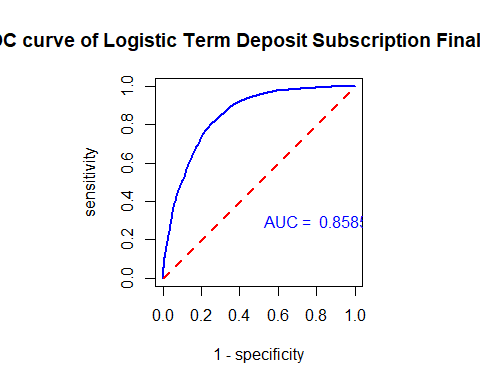
\includegraphics{Bank_files/figure-latex/unnamed-chunk-29-1.pdf}

\begin{Shaded}
\begin{Highlighting}[]
\CommentTok{\# Creating an initial model ROC curve for sensitivity and (1{-}specificity)}
\DocumentationTok{\#\# 5{-}fold CV}
\ControlFlowTok{for}\NormalTok{ (i }\ControlFlowTok{in} \DecValTok{1}\SpecialCharTok{:}\DecValTok{5}\NormalTok{)\{}
\NormalTok{  valid.id }\OtherTok{=}\NormalTok{ ((i}\DecValTok{{-}1}\NormalTok{)}\SpecialCharTok{*}\NormalTok{n0 }\SpecialCharTok{+} \DecValTok{1}\NormalTok{)}\SpecialCharTok{:}\NormalTok{(i}\SpecialCharTok{*}\NormalTok{n0)}
\NormalTok{  valid.data }\OtherTok{=}\NormalTok{ training[valid.id,]}
\NormalTok{  train.data }\OtherTok{=}\NormalTok{ training[}\SpecialCharTok{{-}}\NormalTok{valid.id,]}
\NormalTok{  train.model }\OtherTok{=} \FunctionTok{glm}\NormalTok{(y.subscribe }\SpecialCharTok{\textasciitilde{}}\NormalTok{ age }\SpecialCharTok{+}\NormalTok{ day }\SpecialCharTok{+}\NormalTok{ grp.job }\SpecialCharTok{+}\NormalTok{ marital }\SpecialCharTok{+}\NormalTok{ education }\SpecialCharTok{+}\NormalTok{ housing }\SpecialCharTok{+}\NormalTok{ loan }\SpecialCharTok{+}\NormalTok{ contact }\SpecialCharTok{+}\NormalTok{ grp.duration }\SpecialCharTok{+}\NormalTok{ grp.campaign }\SpecialCharTok{+}\NormalTok{ grp.pdays }\SpecialCharTok{+}\NormalTok{ grp.previous, }\AttributeTok{family =}\NormalTok{ binomial, }\AttributeTok{data =}\NormalTok{ train.data)}
\DocumentationTok{\#\#\#\#}
\NormalTok{  pred.prob }\OtherTok{=} \FunctionTok{predict.glm}\NormalTok{(train.model, valid.data, }\AttributeTok{type =} \StringTok{"response"}\NormalTok{)}
  \CommentTok{\# define confusion matrix and accuracy}
  \ControlFlowTok{for}\NormalTok{(j }\ControlFlowTok{in} \DecValTok{1}\SpecialCharTok{:}\DecValTok{20}\NormalTok{)\{}
    \CommentTok{\#pred.subscribe = rep(0,length(pred.prob))}
\NormalTok{    valid.data}\SpecialCharTok{$}\NormalTok{pred.subscribe }\OtherTok{=} \FunctionTok{as.numeric}\NormalTok{(pred.prob }\SpecialCharTok{\textgreater{}}\NormalTok{ cut}\FloatTok{.0}\NormalTok{ff.prob[j])}
\NormalTok{    a11 }\OtherTok{=} \FunctionTok{sum}\NormalTok{(valid.data}\SpecialCharTok{$}\NormalTok{pred.subscribe }\SpecialCharTok{==}\NormalTok{ valid.data}\SpecialCharTok{$}\NormalTok{y.subscribe)}
\NormalTok{    pred.accuracy[i,j] }\OtherTok{=}\NormalTok{ a11}\SpecialCharTok{/}\FunctionTok{length}\NormalTok{(pred.prob)}
\NormalTok{  \}}
\NormalTok{\}}

\NormalTok{test.model }\OtherTok{=} \FunctionTok{glm}\NormalTok{(y.subscribe }\SpecialCharTok{\textasciitilde{}}\NormalTok{ age }\SpecialCharTok{+}\NormalTok{ day }\SpecialCharTok{+}\NormalTok{ grp.job }\SpecialCharTok{+}\NormalTok{ marital }\SpecialCharTok{+}\NormalTok{ education }\SpecialCharTok{+}\NormalTok{ housing }\SpecialCharTok{+}\NormalTok{ loan }\SpecialCharTok{+}\NormalTok{ contact }\SpecialCharTok{+}\NormalTok{ grp.duration }\SpecialCharTok{+}\NormalTok{ grp.campaign }\SpecialCharTok{+}\NormalTok{ grp.pdays }\SpecialCharTok{+}\NormalTok{ grp.previous, }\AttributeTok{family =} \FunctionTok{binomial}\NormalTok{(}\AttributeTok{link =}\NormalTok{ logit), }\AttributeTok{data =}\NormalTok{ training)}
\NormalTok{newBankingTestingData }\OtherTok{=} \FunctionTok{data.frame}\NormalTok{(}\AttributeTok{age=}\NormalTok{ testing}\SpecialCharTok{$}\NormalTok{age, }\AttributeTok{day=}\NormalTok{ testing}\SpecialCharTok{$}\NormalTok{day, }\AttributeTok{grp.job=}\NormalTok{ testing}\SpecialCharTok{$}\NormalTok{grp.job, }\AttributeTok{marital=}\NormalTok{ testing}\SpecialCharTok{$}\NormalTok{marital, }\AttributeTok{education=}\NormalTok{ testing}\SpecialCharTok{$}\NormalTok{education, }\AttributeTok{housing=}\NormalTok{ testing}\SpecialCharTok{$}\NormalTok{housing, }\AttributeTok{loan=}\NormalTok{ testing}\SpecialCharTok{$}\NormalTok{loan, }\AttributeTok{contact=}\NormalTok{ testing}\SpecialCharTok{$}\NormalTok{contact, }\AttributeTok{grp.duration=}\NormalTok{ testing}\SpecialCharTok{$}\NormalTok{grp.duration, }\AttributeTok{grp.campaign=}\NormalTok{ testing}\SpecialCharTok{$}\NormalTok{grp.campaign, }\AttributeTok{grp.pdays=}\NormalTok{ testing}\SpecialCharTok{$}\NormalTok{grp.pdays, }\AttributeTok{grp.previous=}\NormalTok{ testing}\SpecialCharTok{$}\NormalTok{grp.previous)}

\NormalTok{pred.prob.test }\OtherTok{=} \FunctionTok{predict.glm}\NormalTok{(test.model, newBankingTestingData, }\AttributeTok{type =} \StringTok{"response"}\NormalTok{)}

\NormalTok{cut.off.seq }\OtherTok{=} \FunctionTok{seq}\NormalTok{(}\FloatTok{0.01}\NormalTok{, }\FloatTok{0.99}\NormalTok{, }\AttributeTok{length =} \DecValTok{100}\NormalTok{)}
\NormalTok{sensitivity.vec }\OtherTok{=} \ConstantTok{NULL}
\NormalTok{specificity.vec }\OtherTok{=} \ConstantTok{NULL}
\ControlFlowTok{for}\NormalTok{ (i }\ControlFlowTok{in} \DecValTok{1}\SpecialCharTok{:}\DecValTok{100}\NormalTok{)\{}
\NormalTok{  testing}\SpecialCharTok{$}\NormalTok{test.subscribe }\OtherTok{=} \FunctionTok{as.numeric}\NormalTok{(pred.prob.test }\SpecialCharTok{\textgreater{}}\NormalTok{ cut.off.seq[i])}
\DocumentationTok{\#\#\# components for defining various measures}
\NormalTok{p0.a0 }\OtherTok{=} \FunctionTok{sum}\NormalTok{(testing}\SpecialCharTok{$}\NormalTok{test.subscribe }\SpecialCharTok{==}\DecValTok{0} \SpecialCharTok{\&}\NormalTok{ testing}\SpecialCharTok{$}\NormalTok{y.subscribe }\SpecialCharTok{==}\DecValTok{0}\NormalTok{)}
\NormalTok{p0.a1 }\OtherTok{=} \FunctionTok{sum}\NormalTok{(testing}\SpecialCharTok{$}\NormalTok{test.subscribe }\SpecialCharTok{==}\DecValTok{0} \SpecialCharTok{\&}\NormalTok{ testing}\SpecialCharTok{$}\NormalTok{y.subscribe }\SpecialCharTok{==}\DecValTok{1}\NormalTok{)}
\NormalTok{p1.a0 }\OtherTok{=} \FunctionTok{sum}\NormalTok{(testing}\SpecialCharTok{$}\NormalTok{test.subscribe }\SpecialCharTok{==}\DecValTok{1} \SpecialCharTok{\&}\NormalTok{ testing}\SpecialCharTok{$}\NormalTok{y.subscribe }\SpecialCharTok{==}\DecValTok{0}\NormalTok{)}
\NormalTok{p1.a1 }\OtherTok{=} \FunctionTok{sum}\NormalTok{(testing}\SpecialCharTok{$}\NormalTok{test.subscribe }\SpecialCharTok{==}\DecValTok{1} \SpecialCharTok{\&}\NormalTok{ testing}\SpecialCharTok{$}\NormalTok{y.subscribe }\SpecialCharTok{==}\DecValTok{1}\NormalTok{)}
\DocumentationTok{\#\#\#}
\NormalTok{sensitivity.vec[i] }\OtherTok{=}\NormalTok{ p1.a1 }\SpecialCharTok{/}\NormalTok{ (p1.a1 }\SpecialCharTok{+}\NormalTok{ p0.a1)}
\NormalTok{specificity.vec[i] }\OtherTok{=}\NormalTok{ p0.a0 }\SpecialCharTok{/}\NormalTok{ (p0.a0 }\SpecialCharTok{+}\NormalTok{ p1.a0)}
\NormalTok{\}}
\NormalTok{one.minus.spec }\OtherTok{=} \FunctionTok{c}\NormalTok{(}\DecValTok{1}\NormalTok{,}\DecValTok{1} \SpecialCharTok{{-}}\NormalTok{ specificity.vec)}
\NormalTok{sens.vec }\OtherTok{=} \FunctionTok{c}\NormalTok{(}\DecValTok{1}\NormalTok{,sensitivity.vec)}
\DocumentationTok{\#\#}
\FunctionTok{par}\NormalTok{(}\AttributeTok{pty =} \StringTok{"s"}\NormalTok{)   }\CommentTok{\# make a square figure}
\FunctionTok{plot}\NormalTok{(one.minus.spec, sens.vec, }\AttributeTok{type =} \StringTok{"l"}\NormalTok{, }\AttributeTok{xlim =} \FunctionTok{c}\NormalTok{(}\DecValTok{0}\NormalTok{,}\DecValTok{1}\NormalTok{),}
     \AttributeTok{xlab =}\StringTok{"1 {-} specificity"}\NormalTok{,}
     \AttributeTok{ylab =} \StringTok{"sensitivity"}\NormalTok{,}
     \AttributeTok{main =} \StringTok{"ROC curve of Logistic Term Deposit Subscription Initial Model"}\NormalTok{,}
     \AttributeTok{lwd =} \DecValTok{2}\NormalTok{,}
     \AttributeTok{col =} \StringTok{"blue"}\NormalTok{, )}
\FunctionTok{segments}\NormalTok{(}\DecValTok{0}\NormalTok{,}\DecValTok{0}\NormalTok{,}\DecValTok{1}\NormalTok{,}\DecValTok{1}\NormalTok{, }\AttributeTok{col =} \StringTok{"red"}\NormalTok{, }\AttributeTok{lty =} \DecValTok{2}\NormalTok{, }\AttributeTok{lwd =} \DecValTok{2}\NormalTok{)}
\NormalTok{AUC }\OtherTok{=} \FunctionTok{round}\NormalTok{(}\FunctionTok{sum}\NormalTok{(sens.vec}\SpecialCharTok{*}\NormalTok{(one.minus.spec[}\SpecialCharTok{{-}}\DecValTok{101}\NormalTok{]}\SpecialCharTok{{-}}\NormalTok{one.minus.spec[}\SpecialCharTok{{-}}\DecValTok{1}\NormalTok{])),}\DecValTok{4}\NormalTok{)}
\FunctionTok{text}\NormalTok{(}\FloatTok{0.8}\NormalTok{, }\FloatTok{0.3}\NormalTok{, }\FunctionTok{paste}\NormalTok{(}\StringTok{"AUC = "}\NormalTok{, AUC), }\AttributeTok{col =} \StringTok{"blue"}\NormalTok{)}
\end{Highlighting}
\end{Shaded}

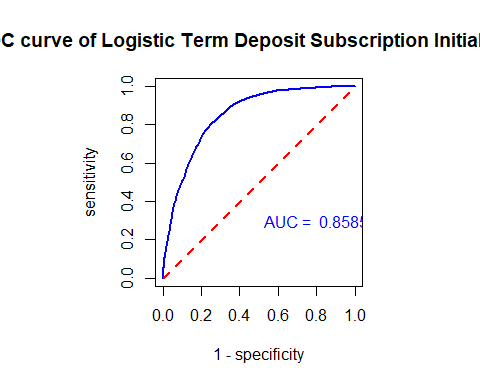
\includegraphics{Bank_files/figure-latex/unnamed-chunk-30-1.pdf}

\begin{Shaded}
\begin{Highlighting}[]
\CommentTok{\# Creating a reduced model ROC curve for sensitivity and (1{-}specificity)}
\DocumentationTok{\#\# 5{-}fold CV}
\ControlFlowTok{for}\NormalTok{ (i }\ControlFlowTok{in} \DecValTok{1}\SpecialCharTok{:}\DecValTok{5}\NormalTok{)\{}
\NormalTok{  valid.id }\OtherTok{=}\NormalTok{ ((i}\DecValTok{{-}1}\NormalTok{)}\SpecialCharTok{*}\NormalTok{n0 }\SpecialCharTok{+} \DecValTok{1}\NormalTok{)}\SpecialCharTok{:}\NormalTok{(i}\SpecialCharTok{*}\NormalTok{n0)}
\NormalTok{  valid.data }\OtherTok{=}\NormalTok{ training[valid.id,]}
\NormalTok{  train.data }\OtherTok{=}\NormalTok{ training[}\SpecialCharTok{{-}}\NormalTok{valid.id,]}
\NormalTok{  train.model }\OtherTok{=} \FunctionTok{glm}\NormalTok{(y.subscribe }\SpecialCharTok{\textasciitilde{}}\NormalTok{ day }\SpecialCharTok{+}\NormalTok{ grp.job }\SpecialCharTok{+}\NormalTok{ marital }\SpecialCharTok{+}\NormalTok{ housing }\SpecialCharTok{+}\NormalTok{ loan }\SpecialCharTok{+}\NormalTok{ contact }\SpecialCharTok{+}\NormalTok{ grp.duration }\SpecialCharTok{+}\NormalTok{ grp.campaign }\SpecialCharTok{+}\NormalTok{ grp.previous, }\AttributeTok{family =} \FunctionTok{binomial}\NormalTok{(}\AttributeTok{link =}\NormalTok{ logit), }\AttributeTok{data =}\NormalTok{ train.data)}
\DocumentationTok{\#\#\#\#}
\NormalTok{  pred.prob }\OtherTok{=} \FunctionTok{predict.glm}\NormalTok{(train.model, valid.data, }\AttributeTok{type =} \StringTok{"response"}\NormalTok{)}
  \CommentTok{\# define confusion matrix and accuracy}
  \ControlFlowTok{for}\NormalTok{(j }\ControlFlowTok{in} \DecValTok{1}\SpecialCharTok{:}\DecValTok{20}\NormalTok{)\{}
    \CommentTok{\#pred.subscribe = rep(0,length(pred.prob))}
\NormalTok{    valid.data}\SpecialCharTok{$}\NormalTok{pred.subscribe }\OtherTok{=} \FunctionTok{as.numeric}\NormalTok{(pred.prob }\SpecialCharTok{\textgreater{}}\NormalTok{ cut}\FloatTok{.0}\NormalTok{ff.prob[j])}
\NormalTok{    a11 }\OtherTok{=} \FunctionTok{sum}\NormalTok{(valid.data}\SpecialCharTok{$}\NormalTok{pred.subscribe }\SpecialCharTok{==}\NormalTok{ valid.data}\SpecialCharTok{$}\NormalTok{y.subscribe)}
\NormalTok{    pred.accuracy[i,j] }\OtherTok{=}\NormalTok{ a11}\SpecialCharTok{/}\FunctionTok{length}\NormalTok{(pred.prob)}
\NormalTok{  \}}
\NormalTok{\}}

\NormalTok{test.model }\OtherTok{=} \FunctionTok{glm}\NormalTok{(y.subscribe }\SpecialCharTok{\textasciitilde{}}\NormalTok{ day }\SpecialCharTok{+}\NormalTok{ grp.job }\SpecialCharTok{+}\NormalTok{ marital }\SpecialCharTok{+}\NormalTok{ housing }\SpecialCharTok{+}\NormalTok{ loan }\SpecialCharTok{+}\NormalTok{ contact }\SpecialCharTok{+}\NormalTok{ grp.duration }\SpecialCharTok{+}\NormalTok{ grp.campaign }\SpecialCharTok{+}\NormalTok{ grp.previous, }\AttributeTok{family =} \FunctionTok{binomial}\NormalTok{(}\AttributeTok{link =}\NormalTok{ logit), }\AttributeTok{data =}\NormalTok{ training)}
\NormalTok{newBankingTestingData }\OtherTok{=} \FunctionTok{data.frame}\NormalTok{(}\AttributeTok{day=}\NormalTok{ testing}\SpecialCharTok{$}\NormalTok{day, }\AttributeTok{grp.job=}\NormalTok{ testing}\SpecialCharTok{$}\NormalTok{grp.job, }\AttributeTok{marital=}\NormalTok{ testing}\SpecialCharTok{$}\NormalTok{marital, }\AttributeTok{housing=}\NormalTok{ testing}\SpecialCharTok{$}\NormalTok{housing, }\AttributeTok{loan=}\NormalTok{ testing}\SpecialCharTok{$}\NormalTok{loan, }\AttributeTok{contact=}\NormalTok{ testing}\SpecialCharTok{$}\NormalTok{contact, }\AttributeTok{grp.duration=}\NormalTok{ testing}\SpecialCharTok{$}\NormalTok{grp.duration, }\AttributeTok{grp.campaign=}\NormalTok{ testing}\SpecialCharTok{$}\NormalTok{grp.campaign, }\AttributeTok{grp.previous=}\NormalTok{ testing}\SpecialCharTok{$}\NormalTok{grp.previous)}

\NormalTok{pred.prob.test }\OtherTok{=} \FunctionTok{predict.glm}\NormalTok{(test.model, newBankingTestingData, }\AttributeTok{type =} \StringTok{"response"}\NormalTok{)}

\NormalTok{cut.off.seq }\OtherTok{=} \FunctionTok{seq}\NormalTok{(}\FloatTok{0.01}\NormalTok{, }\FloatTok{0.99}\NormalTok{, }\AttributeTok{length =} \DecValTok{100}\NormalTok{)}
\NormalTok{sensitivity.vec }\OtherTok{=} \ConstantTok{NULL}
\NormalTok{specificity.vec }\OtherTok{=} \ConstantTok{NULL}
\ControlFlowTok{for}\NormalTok{ (i }\ControlFlowTok{in} \DecValTok{1}\SpecialCharTok{:}\DecValTok{100}\NormalTok{)\{}
\NormalTok{  testing}\SpecialCharTok{$}\NormalTok{test.subscribe }\OtherTok{=} \FunctionTok{as.numeric}\NormalTok{(pred.prob.test }\SpecialCharTok{\textgreater{}}\NormalTok{ cut.off.seq[i])}
\DocumentationTok{\#\#\# components for defining various measures}
\NormalTok{p0.a0 }\OtherTok{=} \FunctionTok{sum}\NormalTok{(testing}\SpecialCharTok{$}\NormalTok{test.subscribe }\SpecialCharTok{==}\DecValTok{0} \SpecialCharTok{\&}\NormalTok{ testing}\SpecialCharTok{$}\NormalTok{y.subscribe }\SpecialCharTok{==}\DecValTok{0}\NormalTok{)}
\NormalTok{p0.a1 }\OtherTok{=} \FunctionTok{sum}\NormalTok{(testing}\SpecialCharTok{$}\NormalTok{test.subscribe }\SpecialCharTok{==}\DecValTok{0} \SpecialCharTok{\&}\NormalTok{ testing}\SpecialCharTok{$}\NormalTok{y.subscribe }\SpecialCharTok{==}\DecValTok{1}\NormalTok{)}
\NormalTok{p1.a0 }\OtherTok{=} \FunctionTok{sum}\NormalTok{(testing}\SpecialCharTok{$}\NormalTok{test.subscribe }\SpecialCharTok{==}\DecValTok{1} \SpecialCharTok{\&}\NormalTok{ testing}\SpecialCharTok{$}\NormalTok{y.subscribe }\SpecialCharTok{==}\DecValTok{0}\NormalTok{)}
\NormalTok{p1.a1 }\OtherTok{=} \FunctionTok{sum}\NormalTok{(testing}\SpecialCharTok{$}\NormalTok{test.subscribe }\SpecialCharTok{==}\DecValTok{1} \SpecialCharTok{\&}\NormalTok{ testing}\SpecialCharTok{$}\NormalTok{y.subscribe }\SpecialCharTok{==}\DecValTok{1}\NormalTok{)}
\DocumentationTok{\#\#\#}
\NormalTok{sensitivity.vec[i] }\OtherTok{=}\NormalTok{ p1.a1 }\SpecialCharTok{/}\NormalTok{ (p1.a1 }\SpecialCharTok{+}\NormalTok{ p0.a1)}
\NormalTok{specificity.vec[i] }\OtherTok{=}\NormalTok{ p0.a0 }\SpecialCharTok{/}\NormalTok{ (p0.a0 }\SpecialCharTok{+}\NormalTok{ p1.a0)}
\NormalTok{\}}
\NormalTok{one.minus.spec }\OtherTok{=} \FunctionTok{c}\NormalTok{(}\DecValTok{1}\NormalTok{,}\DecValTok{1} \SpecialCharTok{{-}}\NormalTok{ specificity.vec)}
\NormalTok{sens.vec }\OtherTok{=} \FunctionTok{c}\NormalTok{(}\DecValTok{1}\NormalTok{,sensitivity.vec)}
\DocumentationTok{\#\#}
\FunctionTok{par}\NormalTok{(}\AttributeTok{pty =} \StringTok{"s"}\NormalTok{)   }\CommentTok{\# make a square figure}
\FunctionTok{plot}\NormalTok{(one.minus.spec, sens.vec, }\AttributeTok{type =} \StringTok{"l"}\NormalTok{, }\AttributeTok{xlim =} \FunctionTok{c}\NormalTok{(}\DecValTok{0}\NormalTok{,}\DecValTok{1}\NormalTok{),}
     \AttributeTok{xlab =}\StringTok{"1 {-} specificity"}\NormalTok{,}
     \AttributeTok{ylab =} \StringTok{"sensitivity"}\NormalTok{,}
     \AttributeTok{main =} \StringTok{"ROC curve of Logistic Term Deposit Subscription Reduced Model"}\NormalTok{,}
     \AttributeTok{lwd =} \DecValTok{2}\NormalTok{,}
     \AttributeTok{col =} \StringTok{"blue"}\NormalTok{, )}
\FunctionTok{segments}\NormalTok{(}\DecValTok{0}\NormalTok{,}\DecValTok{0}\NormalTok{,}\DecValTok{1}\NormalTok{,}\DecValTok{1}\NormalTok{, }\AttributeTok{col =} \StringTok{"red"}\NormalTok{, }\AttributeTok{lty =} \DecValTok{2}\NormalTok{, }\AttributeTok{lwd =} \DecValTok{2}\NormalTok{)}
\NormalTok{AUC }\OtherTok{=} \FunctionTok{round}\NormalTok{(}\FunctionTok{sum}\NormalTok{(sens.vec}\SpecialCharTok{*}\NormalTok{(one.minus.spec[}\SpecialCharTok{{-}}\DecValTok{101}\NormalTok{]}\SpecialCharTok{{-}}\NormalTok{one.minus.spec[}\SpecialCharTok{{-}}\DecValTok{1}\NormalTok{])),}\DecValTok{4}\NormalTok{)}
\FunctionTok{text}\NormalTok{(}\FloatTok{0.8}\NormalTok{, }\FloatTok{0.3}\NormalTok{, }\FunctionTok{paste}\NormalTok{(}\StringTok{"AUC = "}\NormalTok{, AUC), }\AttributeTok{col =} \StringTok{"blue"}\NormalTok{)}
\end{Highlighting}
\end{Shaded}

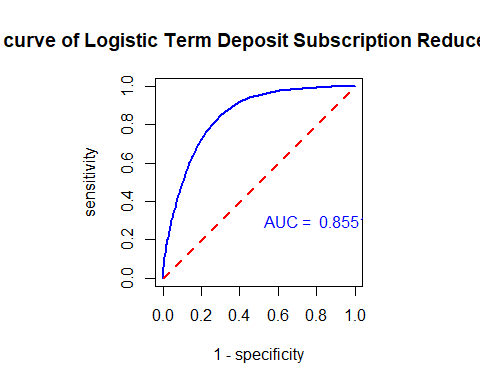
\includegraphics{Bank_files/figure-latex/unnamed-chunk-31-1.pdf}

The area under the curve (AUC) for the reduced model and the ROC curve
is less than the other two graphs. Higher AUC indicates the model for
that curve is better. Therefore, the reduced model is not the best model
to use and is no longer considered. But, it should be noted that it is
not far off the other 2 models.

Looking at the initial and final models, they have the same curve since
both models contain all feature variables used in the initial model. Out
of these other two models, the final model works better compared to the
initial model. It has been proven to be accurate in modeling
performance, has high specificity, and its ROC curve is remaining away
from the 45 degrees mark. Plus, the AUC is fairly high at .8525, even
though the initial model has the same score. \#\# Results and Conclusion
Now that we have chosed the best model out of the three candidate
models, we can use it to predict whether or not a client has subscribed
a term deposit. Using out optimal cut-off of .57

\begin{Shaded}
\begin{Highlighting}[]
\CommentTok{\# Predicting Response Value for Banking Client Given Variable Values for the Final Model}
\NormalTok{pdata }\OtherTok{=} \FunctionTok{data.frame}\NormalTok{(}\AttributeTok{age=}\FunctionTok{c}\NormalTok{(}\DecValTok{25}\NormalTok{,}\DecValTok{64}\NormalTok{),}
                       \AttributeTok{day =} \FunctionTok{c}\NormalTok{(}\DecValTok{5}\NormalTok{,}\DecValTok{5}\NormalTok{),}
                       \AttributeTok{grp.job =} \FunctionTok{c}\NormalTok{(}\StringTok{"1"}\NormalTok{,}\StringTok{"2"}\NormalTok{),}
                       \AttributeTok{marital =} \FunctionTok{c}\NormalTok{(}\StringTok{"0"}\NormalTok{,}\StringTok{"1"}\NormalTok{),}
                       \AttributeTok{education =} \FunctionTok{c}\NormalTok{(}\StringTok{"2"}\NormalTok{,}\StringTok{"0"}\NormalTok{),}
                       \AttributeTok{housing =} \FunctionTok{c}\NormalTok{(}\StringTok{"1"}\NormalTok{,}\StringTok{"1"}\NormalTok{),}
                       \AttributeTok{loan =} \FunctionTok{c}\NormalTok{(}\StringTok{"0"}\NormalTok{,}\StringTok{"1"}\NormalTok{),}
                       \AttributeTok{contact =} \FunctionTok{c}\NormalTok{(}\StringTok{"0"}\NormalTok{,}\StringTok{"0"}\NormalTok{),}
                       \AttributeTok{grp.duration =} \FunctionTok{c}\NormalTok{(}\StringTok{"0"}\NormalTok{,}\StringTok{"1"}\NormalTok{),}
                       \AttributeTok{grp.campaign =} \FunctionTok{c}\NormalTok{(}\StringTok{"1"}\NormalTok{,}\StringTok{"0"}\NormalTok{),}
                       \AttributeTok{grp.pdays =} \FunctionTok{c}\NormalTok{(}\StringTok{"1"}\NormalTok{,}\StringTok{"2"}\NormalTok{),}
                      \AttributeTok{poutcome=}\FunctionTok{c}\NormalTok{(}\StringTok{"0"}\NormalTok{,}\StringTok{"0"}\NormalTok{),}
                       \AttributeTok{grp.previous =} \FunctionTok{c}\NormalTok{(}\StringTok{"1"}\NormalTok{,}\StringTok{"2"}\NormalTok{))}
          



\NormalTok{pred.success.prob }\OtherTok{=} \FunctionTok{predict}\NormalTok{(final.model, }\AttributeTok{newdata =}\NormalTok{ pdata, }\AttributeTok{type=}\StringTok{"response"}\NormalTok{)}

\DocumentationTok{\#\# threshold probability}
\NormalTok{cut.off.prob }\OtherTok{=} \FloatTok{0.57}
\NormalTok{pred.response }\OtherTok{=} \FunctionTok{ifelse}\NormalTok{(pred.success.prob }\SpecialCharTok{\textgreater{}}\NormalTok{ cut.off.prob, }\DecValTok{1}\NormalTok{, }\DecValTok{0}\NormalTok{)  }\CommentTok{\# This predicts the response}
\NormalTok{pred.response}
\end{Highlighting}
\end{Shaded}

\begin{verbatim}
## 1 2 
## 0 0
\end{verbatim}

\begin{Shaded}
\begin{Highlighting}[]
\CommentTok{\# Add the new predicted response to pdata}

\CommentTok{\#pdata$pred.response \textless{}{-} predict(final.model, newdata = pdata, type = "response")}
\NormalTok{pdata}\SpecialCharTok{$}\NormalTok{Pred.Response }\OtherTok{=}\NormalTok{ pred.response}
\FunctionTok{kable}\NormalTok{(pdata, }\AttributeTok{caption =} \StringTok{"Predicted Value of response variable with the given cut{-}off probability"}\NormalTok{)}
\end{Highlighting}
\end{Shaded}

\begin{longtable}[]{@{}
  >{\raggedleft\arraybackslash}p{(\columnwidth - 26\tabcolsep) * \real{0.0315}}
  >{\raggedleft\arraybackslash}p{(\columnwidth - 26\tabcolsep) * \real{0.0315}}
  >{\raggedright\arraybackslash}p{(\columnwidth - 26\tabcolsep) * \real{0.0630}}
  >{\raggedright\arraybackslash}p{(\columnwidth - 26\tabcolsep) * \real{0.0630}}
  >{\raggedright\arraybackslash}p{(\columnwidth - 26\tabcolsep) * \real{0.0787}}
  >{\raggedright\arraybackslash}p{(\columnwidth - 26\tabcolsep) * \real{0.0630}}
  >{\raggedright\arraybackslash}p{(\columnwidth - 26\tabcolsep) * \real{0.0394}}
  >{\raggedright\arraybackslash}p{(\columnwidth - 26\tabcolsep) * \real{0.0630}}
  >{\raggedright\arraybackslash}p{(\columnwidth - 26\tabcolsep) * \real{0.1024}}
  >{\raggedright\arraybackslash}p{(\columnwidth - 26\tabcolsep) * \real{0.1024}}
  >{\raggedright\arraybackslash}p{(\columnwidth - 26\tabcolsep) * \real{0.0787}}
  >{\raggedright\arraybackslash}p{(\columnwidth - 26\tabcolsep) * \real{0.0709}}
  >{\raggedright\arraybackslash}p{(\columnwidth - 26\tabcolsep) * \real{0.1024}}
  >{\raggedleft\arraybackslash}p{(\columnwidth - 26\tabcolsep) * \real{0.1102}}@{}}
\caption{Predicted Value of response variable with the given cut-off
probability}\tabularnewline
\toprule\noalign{}
\begin{minipage}[b]{\linewidth}\raggedleft
age
\end{minipage} & \begin{minipage}[b]{\linewidth}\raggedleft
day
\end{minipage} & \begin{minipage}[b]{\linewidth}\raggedright
grp.job
\end{minipage} & \begin{minipage}[b]{\linewidth}\raggedright
marital
\end{minipage} & \begin{minipage}[b]{\linewidth}\raggedright
education
\end{minipage} & \begin{minipage}[b]{\linewidth}\raggedright
housing
\end{minipage} & \begin{minipage}[b]{\linewidth}\raggedright
loan
\end{minipage} & \begin{minipage}[b]{\linewidth}\raggedright
contact
\end{minipage} & \begin{minipage}[b]{\linewidth}\raggedright
grp.duration
\end{minipage} & \begin{minipage}[b]{\linewidth}\raggedright
grp.campaign
\end{minipage} & \begin{minipage}[b]{\linewidth}\raggedright
grp.pdays
\end{minipage} & \begin{minipage}[b]{\linewidth}\raggedright
poutcome
\end{minipage} & \begin{minipage}[b]{\linewidth}\raggedright
grp.previous
\end{minipage} & \begin{minipage}[b]{\linewidth}\raggedleft
Pred.Response
\end{minipage} \\
\midrule\noalign{}
\endfirsthead
\toprule\noalign{}
\begin{minipage}[b]{\linewidth}\raggedleft
age
\end{minipage} & \begin{minipage}[b]{\linewidth}\raggedleft
day
\end{minipage} & \begin{minipage}[b]{\linewidth}\raggedright
grp.job
\end{minipage} & \begin{minipage}[b]{\linewidth}\raggedright
marital
\end{minipage} & \begin{minipage}[b]{\linewidth}\raggedright
education
\end{minipage} & \begin{minipage}[b]{\linewidth}\raggedright
housing
\end{minipage} & \begin{minipage}[b]{\linewidth}\raggedright
loan
\end{minipage} & \begin{minipage}[b]{\linewidth}\raggedright
contact
\end{minipage} & \begin{minipage}[b]{\linewidth}\raggedright
grp.duration
\end{minipage} & \begin{minipage}[b]{\linewidth}\raggedright
grp.campaign
\end{minipage} & \begin{minipage}[b]{\linewidth}\raggedright
grp.pdays
\end{minipage} & \begin{minipage}[b]{\linewidth}\raggedright
poutcome
\end{minipage} & \begin{minipage}[b]{\linewidth}\raggedright
grp.previous
\end{minipage} & \begin{minipage}[b]{\linewidth}\raggedleft
Pred.Response
\end{minipage} \\
\midrule\noalign{}
\endhead
\bottomrule\noalign{}
\endlastfoot
25 & 5 & 1 & 0 & 2 & 1 & 0 & 0 & 0 & 1 & 1 & 0 & 1 & 0 \\
64 & 5 & 2 & 1 & 0 & 1 & 1 & 0 & 1 & 0 & 2 & 0 & 2 & 0 \\
\end{longtable}

You can see that neither of the two observations will be subscribing.
More testing can be done with the testing dataset.

\section{Summary and Discussion}\label{summary-and-discussion}

Overall in this project we have done some EDA with linear and logistical
regression to answer two questions: 1. What factors affect the duration
of a call? 2. If we can predict whether a client will subscribe to
direct marketing.

In our modeling we cannot rely on the linear model as the assumption
have be violated and there is no strong evidence to support and claims.
But, in our logistic model we were able to accurately predict whether a
client will subscribe to the marketing. Some more EDA and wrangling is
needed to fit the linear model, or maybe reworking the question is a
more viable solution.

\end{document}
